






\section{Gaussian process submodels}

This package represents a Gaussian process $f\sim \textup{GP}(M,C)$ as a \texttt{GaussianProcess} object which, as you might expect, is a PyMC \texttt{stochastic} whose value is a \texttt{Realization} object. It is not feasible to endow a full \texttt{GaussianProcess} with a \texttt{logp} attribute, so \texttt{GaussianProcess} objects cannot be handled by PyMC's standard MCMC machinery.

However, the evaluation $f(x_*)$ on a mesh $x_*$ is a simple multivariate normal random variable, which can be handled by the standard machinery. If $f(x_*)$ is incorporated in the model as a variable, a minor extension to the standard machinery (section \ref{sec:step-methods}) makes it possible to handle $f$ itself as well.

Pairs of $f$ and $f(x_*)$ variables are created by \texttt{GPSubmodel} objects, which are containers for PyMC variables. \texttt{GaussianProcess} objects can only be incorporated in PyMC probability models via \texttt{GPSubmodel} objects.






\section{Example: nonparametric regression with unknown mean and covariance parameters}\label{sub:BasicMCMC}

A GP submodel is created in \file{examples/gp/PyMCmodel.py} with the following call:
\begin{verbatim}
    sm = gp.GPSubmodel('sm',M,C,fmesh)
\end{verbatim}
There are two stochastic variables in the submodel: \texttt{smf} and \texttt{smf_eval}. The first is the actual Gaussian process $f$: a stochastic variable valued as a \texttt{Realization} object. The second is $f(x_*)$, where $x_*$ is the input argument \texttt{fmesh}.

Once the GP submodel is created, we can create other variables that depend on $f$ and $f(x_*)$. In \file{PyMCmodel.py}, the observation $d$ depends on $f(x_*)$: 
\begin{verbatim}
    d = pymc.Normal('d',mu=smf_eval, tau=1./V, value=init_val, observed=True)
\end{verbatim}
The full probability model is shown as a directed acyclic graph in figure \ref{fig:unobservedModel}. It illustrates the dependency relationships between the variables in a GP submodel.

The file \file{examples/gp/MCMC.py} fits the probability model created in \file{PyMCmodel.py} using MCMC. The `business part' of the file is very simple:
\begin{verbatim}
    GPSampler = MCMC(PyMCmodel)
    GPSampler.isample(iter=5000,burn=1000,thin=100)
\end{verbatim}
Most of the code in the file is devoted to plotting, and its output is shown in figure \ref{fig:MCMCOutput}. Note that after the MCMC run \texttt{GPSampler.trace('sm_f')[:]} yields a sequence of \texttt{Realization} objects, which can be evaluated on new arrays for plotting. GP realizations can even be tallied on disk using the HDF5 backend (see PyMC's user guide).

\begin{figure}
    \centering
        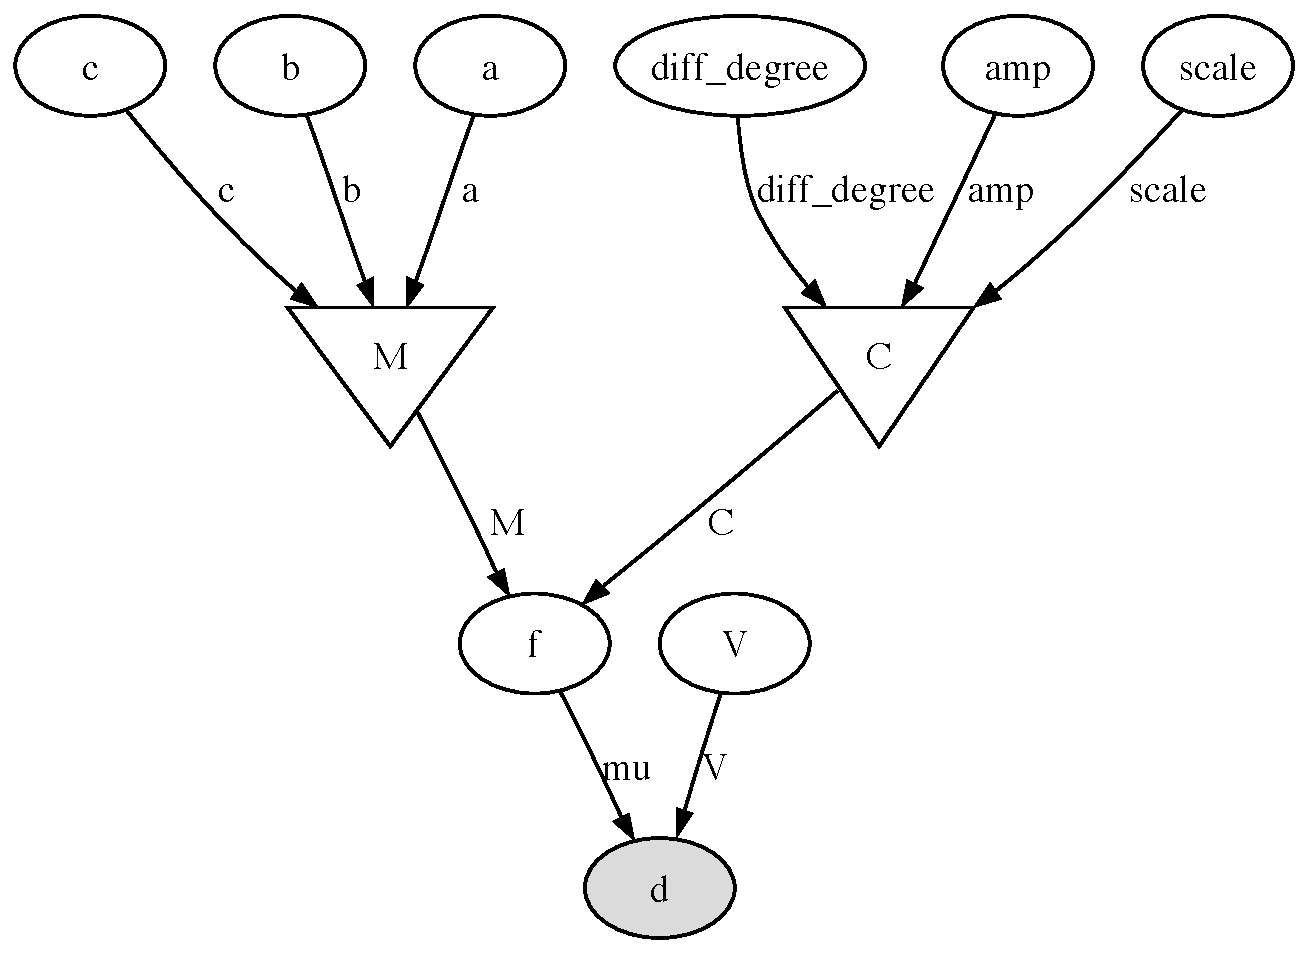
\epsfig{file=figs/unobservedModel.pdf, width=15cm}
    \caption{The PyMC-generated directed acyclic graph representation of the extended nonparametric regression model created by \sffamily{`examples/gp/PyMCModel.py'}. Ellipses represent \texttt{Stochastic} objects (variables whose values are unknown even if their parents' values are known), triangles represent \texttt{Deterministic} objects (variables whose values can be determined if their parents' values are known), and rectangles represent \texttt{Stochastic} objects with the \member{isdata} flag set to \member{True} (data). Rectangles represent potentials. Arrows point from parent to child. The submodel contains the Gaussian process \texttt{sm\_f} and its evaluation \texttt{sm\_f\_eval} on input array \texttt{sm\_mesh}. It also contains the mean \texttt{sm\_M\_eval} of \texttt{sm\_f\_eval} and the lower-triangular Cholesky factor \texttt{sm\_S\_eval} of its covariance matrix, and a potential \texttt{sm_fr_check} that forces that covariance matrix to remain positive definite. The actual covariance evaluation \texttt{sm\_C\_eval} is not needed by the model, but it is exposed for use by Gibbs step methods.}
    \label{fig:unobservedModel}
\end{figure}

\begin{figure}
    \centering
        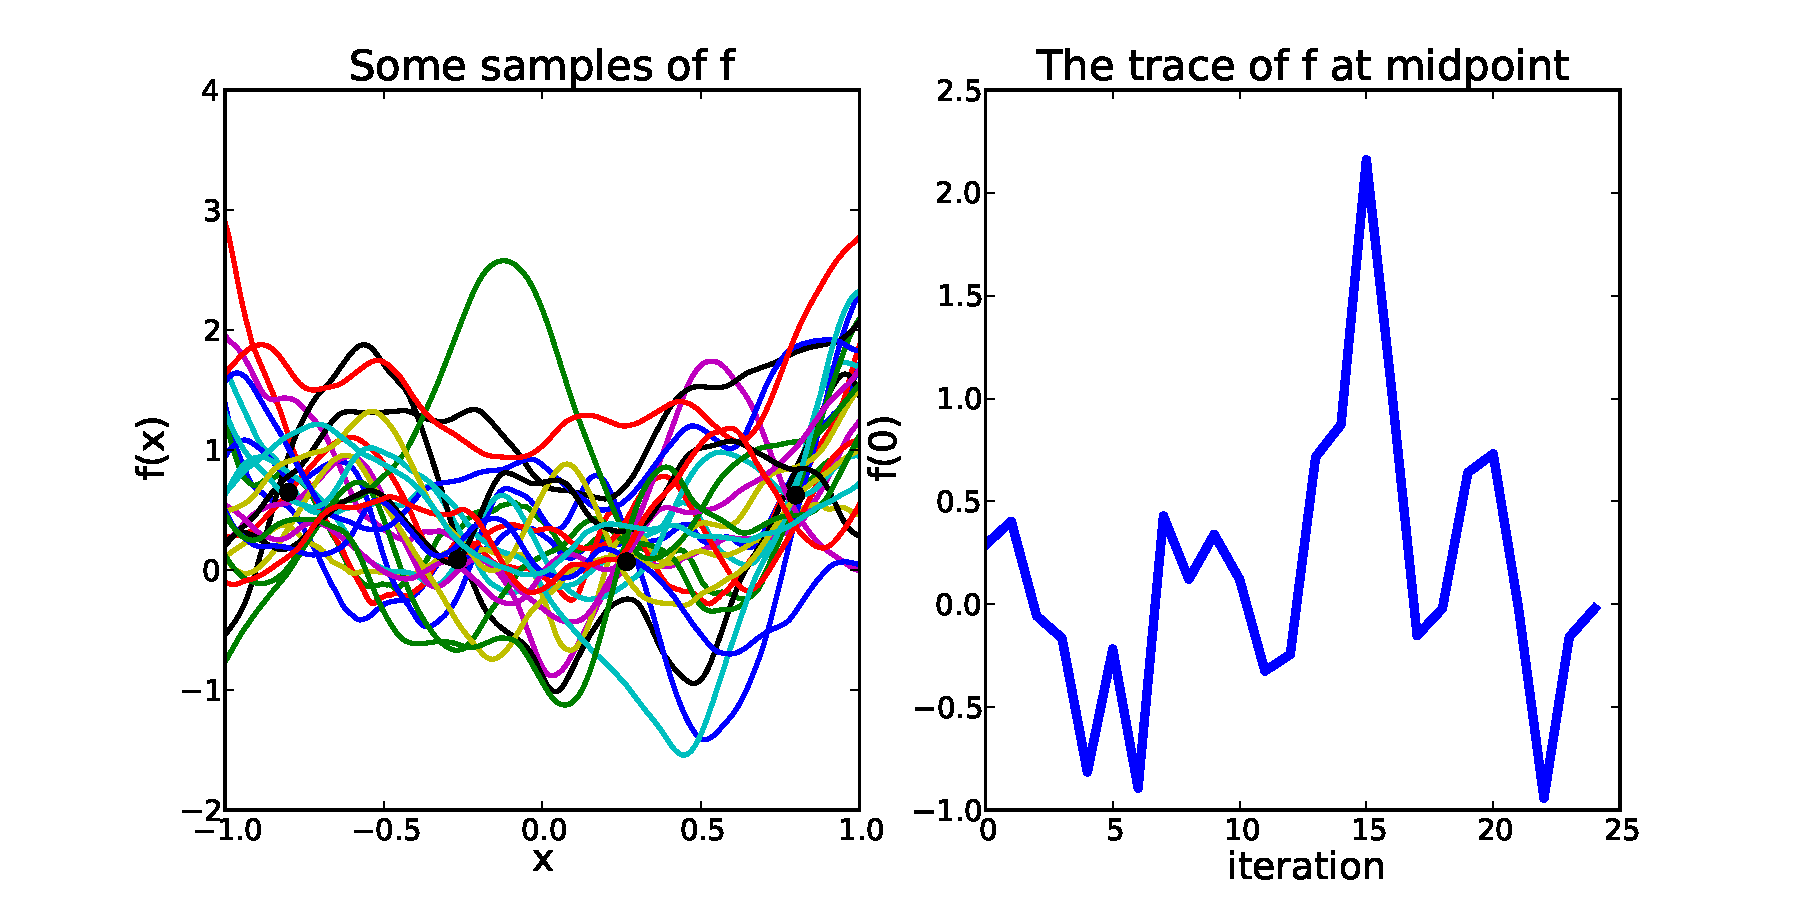
\epsfig{file=figs/gibbsSamples.pdf,width=10cm}
        % 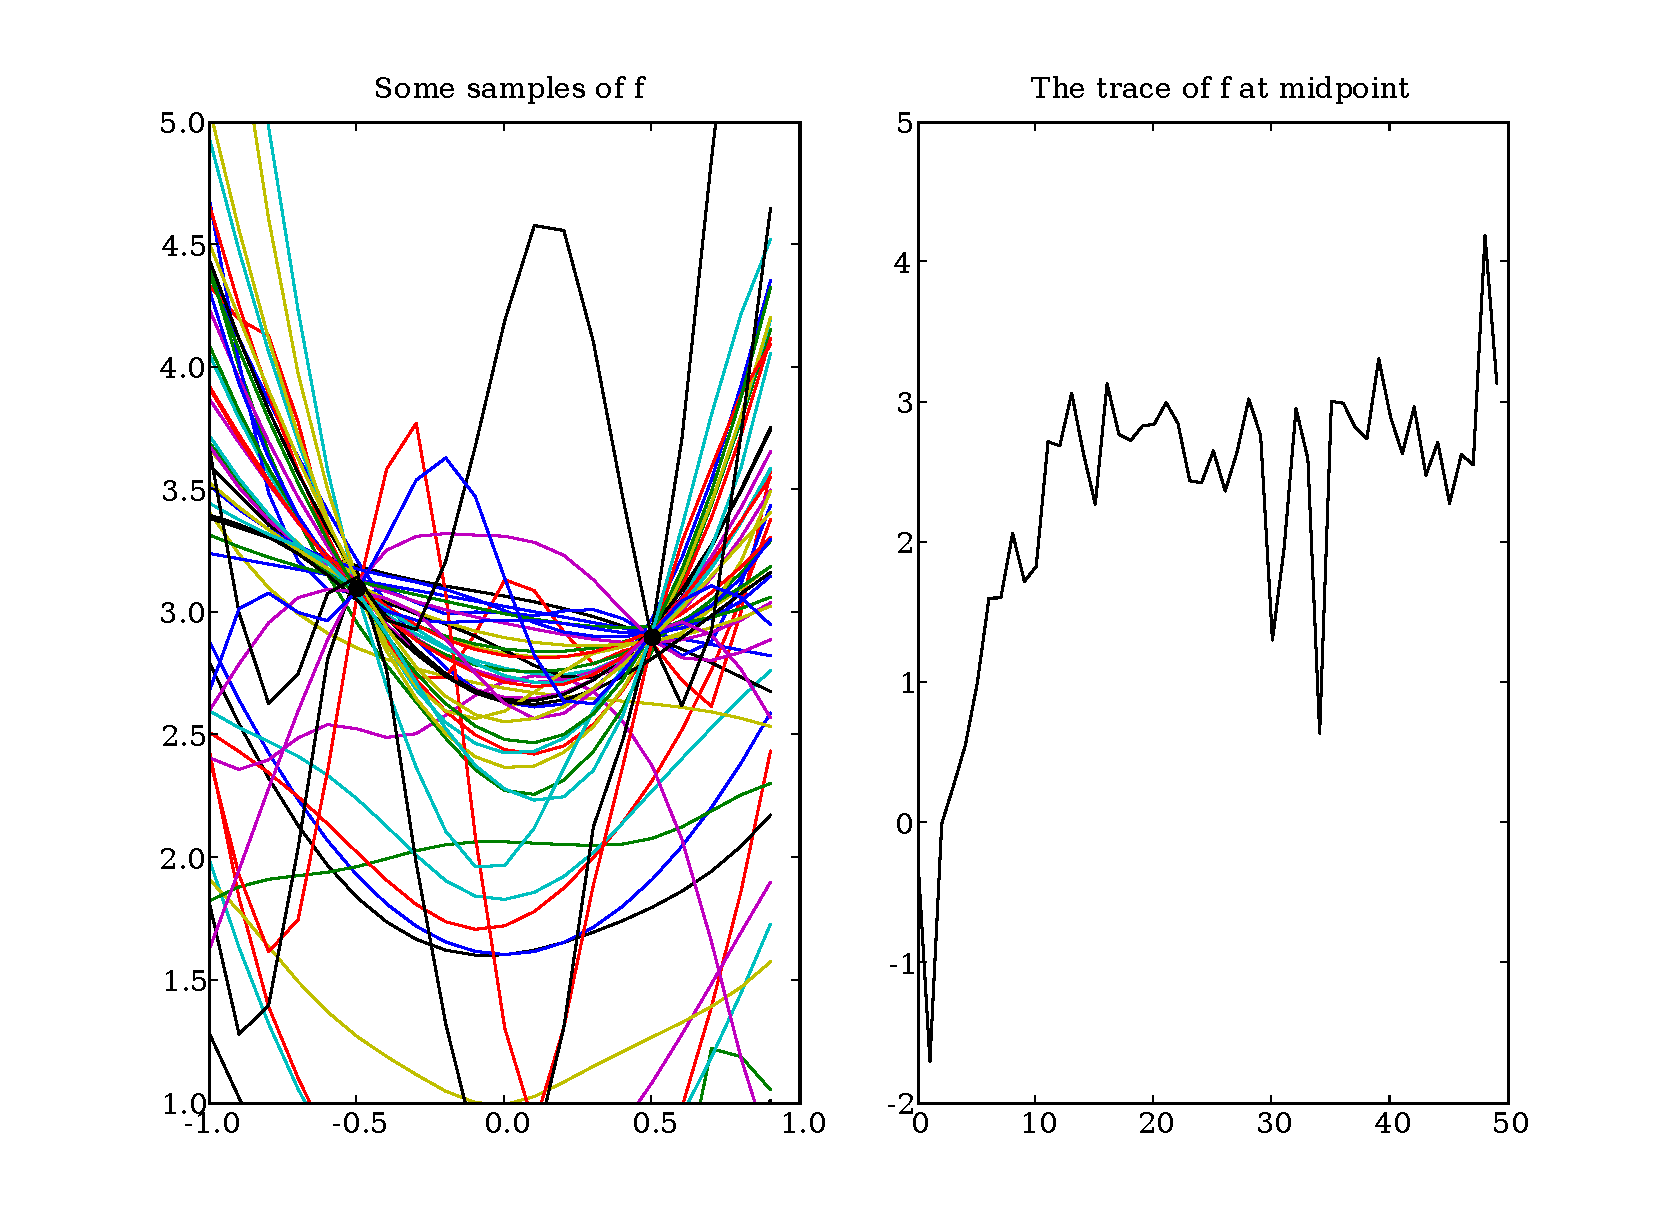
\epsfig{file=figs/metroSamples.pdf,width=10cm}
    \caption{The output of \sffamily{`examples/gp/MCMC.py'}. The left-hand panel shows all the samples generated for the Gaussian process $f$, and the right-hand panel shows the trace of $f(0)$.}
    \label{fig:MCMCOutput}
\end{figure}






\section{Step methods}
\label{sec:step-methods} 
Since $f$ has no \texttt{logp} attribute, the Metropolis-Hastings family of step methods cannot be used to update $f$, $f(x_*)$ or any of their mean or covariance parameters. This package uses a relatively simple work-around that will be described here. Throughout this section, the parents of $f$ are denoted $P$ and the children $K$.


\subsection{Step methods that handle parents of Gaussian processes}
If we could come up with a probability density function for $f$, the Metropolis-Hastings acceptance ratio for a proposed value $P_p$ of the parents \emph{and} a proposed value $\tilde f$ for $f$ would be:
\begin{eqnarray*}
    \frac{p(K|f_p)\ p(f_p|P_p)\ q(P)}{p(K|f)\ p(f|P)\ q(P_p)}
\end{eqnarray*}
where $q$ denotes the proposal density. Now, suppose we proposed a value for $f$ conditional on the proposed values for the parents $P$ \emph{and} conditional on $f(x_*)$. The new acceptance ratio would become
\begin{eqnarray*}
    \frac{p(K|f_p)\ p(f_p|f(x_*), P_p)\ p(f(x_*) | P_p)\ q(f_p|f(x_*),f_p, P_p)\ q(P)}{p(K|f)\ p(f|f(x_*), P)\ p(f(x_*) | P)\ q(f_p|f(x_*),f,P)\ q(P_p)}
\end{eqnarray*}
 We want to avoid computing all terms with $f$ or $f_p$ in the consequent position:
\begin{eqnarray*}
    p(f_p|f(x_*), P),\\ q(f|f(x_*),f_p,P),\\ p(f|f(x_*), P),\\ q(f_p|f(x_*),f,P_p),
\end{eqnarray*}
but all other terms are fine. We can make the problem terms cancel by choosing our proposal distribution as follows:
\begin{eqnarray*}
    q(f_p|f(x_*),f,P_p) = p(f_p|f(x_*), P).
\end{eqnarray*}
In other words, if we propose $f$ from its prior distribution conditional on $f(x_*)$ and its parents whenever we propose $f(x_*)$, we don't have to worry about computing the intractable terms. This argument can be made more rigorous by replacing $f$ with its evaluation at all the points at which we would ever want to know it.

By choosing the same proposal distribution for $\tilde f$ as above, we again avoid having to compute the intractable terms. In other words, every time a value is proposed for a \texttt{GP}'s parent, a value must be proposed for the \texttt{GP}  conditional on its value's evaluation on its mesh, and the prior probability of the \texttt{GP}'s children must be included in the acceptance ratio.

\bigskip
To summarize, any Metropolis-Hastings step method can handle the parents of $f$, as well as $f(x_*)$, if it proposes values for $f$ jointly with its target variable as outlined above. 

This minor alteration can be done using the function \texttt{wrap_metropolis_for_gp_parents}, which takes a subclass of \texttt{Metropolis} as an argument and returns a new step method class with altered \texttt{propose} and \texttt{reject} methods. The function automatically produces modified versions of all Metropolis step methods in PyMC's step method registry (\texttt{Metropolis}, \texttt{AdaptiveMetropolis}, etc.). The modified step methods are automatically assigned to parents of Gaussian processes.

\subsection{Choosing a mesh} 

The mesh points $x_*$ are the points where Metropolis-Hastings step methods can `grab' the value of $f$ to moderate the variance of its proposal distribution. If $x_*$ is an empty array, $f$'s value will be proposed from its prior, and rejection rates are likely to be quite large. If $x_*$ is too dense, on the other hand, computation of the log-probability of $f(x_*)$ will be expensive, as it scales as the cube of the number of points in the mesh.This continuum is illustrated in figure \ref{fig:meshpropose}. Finding the happy medium requires some experimentation.

Another important point to bear in mind is that if $f$'s children depend on its value only via its evaluation on the mesh, the likelihood terms $p(K|f_p)$ and $p(K|f)$ will cancel. In other words, if the mesh is chosen so that $p(K|f)=p(K|f(x_*))$ then the proposed value of $f$ will have no bearing on the acceptance probability of the proposed value of $f(x_*)$ or of the parents $P$. This is the situation in \file{PyMCModel.py}. Such a mesh choice will generally improve the acceptance rate.

\begin{figure}
    \centering
        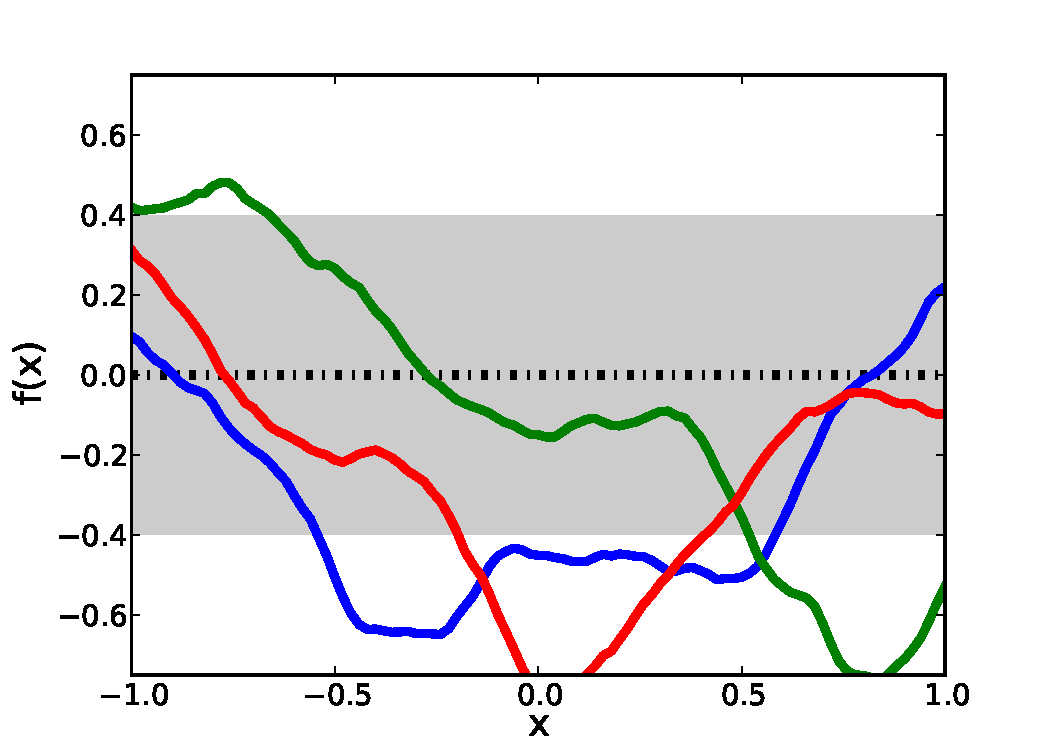
\epsfig{file=figs/nomeshpropose.pdf,width=9cm}
        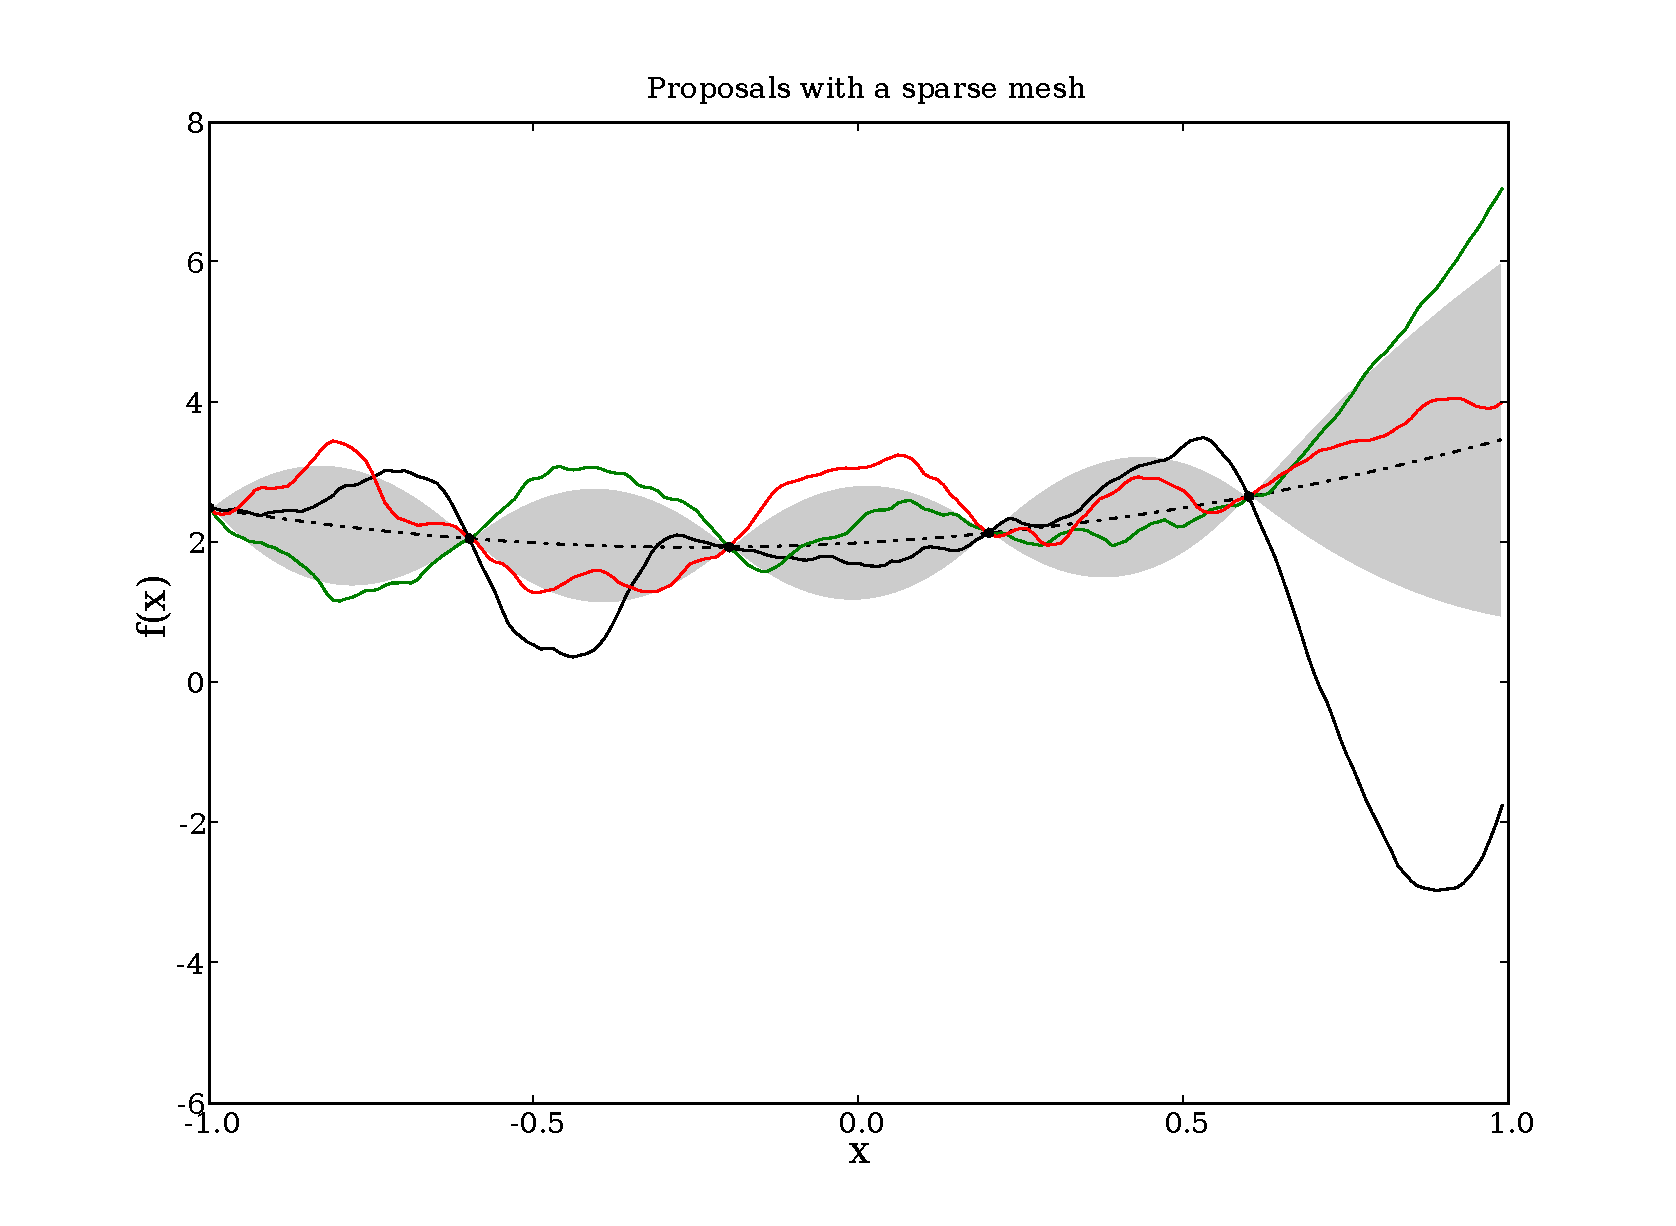
\epsfig{file=figs/lightmeshpropose.pdf,width=9cm}
        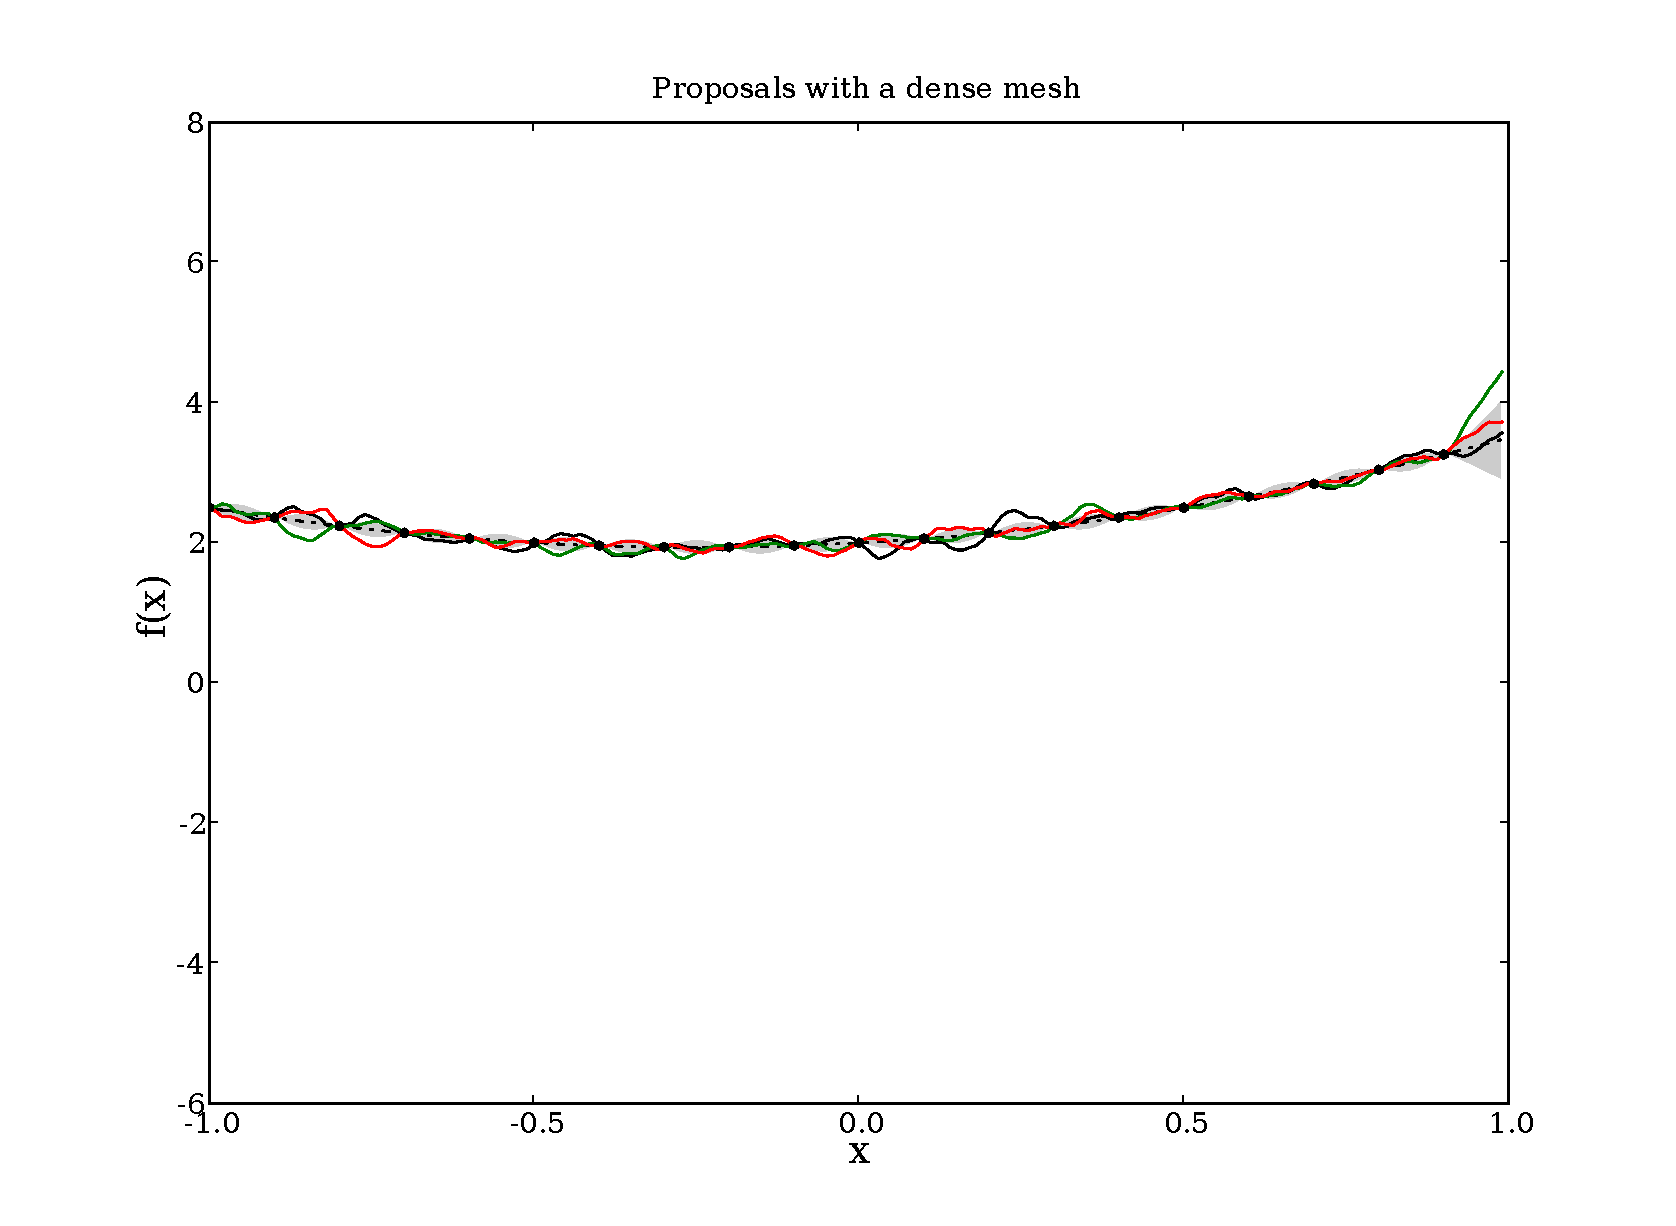
\epsfig{file=figs/densemeshpropose.pdf,width=9cm}
    \caption{Several possible proposals of $f$ (curves) given proposed values for $f(x_*)$ (heavy dots) with no mesh (top), a sparse mesh (middle), and a dense mesh (bottom). Proposal distributions' envelopes are shown as shaded regions, with means shown as broken lines. With no mesh, $f$ is proposed from its prior and the acceptance rate will be very low. A denser mesh permits a high degree of control over $f$, but computing the log-probability will be more expensive.}
    \label{fig:meshpropose}
\end{figure}

\subsection{The \texttt{GPEvaluationGibbs} class} 
If all of $f$'s children $K$, depend on it as follows:
\begin{eqnarray*}
    K_i|f \stackrel{\textup{\tiny ind}}{\sim} \textup{Normal}(f(x_{*i}),V_i)
\end{eqnarray*}
then $f(x_*)$ can be handled by the \texttt{GPEvaluationGibbs} step method. This step method is used in \file{MCMC.py}:
\begin{verbatim}
    GPSampler.use_step_method(gp.GPEvaluationGibbs, GPSampler.submod, GPSampler.V, GPSampler.d)
\end{verbatim}
The initialization arguments are the Gaussian process submodel that contains $f$, the observation variance of $f$'s children, and the children, in this case the vector-valued normal variable $d$. 

\texttt{GPEvaluationGibbs} covers the standard submodel encountered in geostatistics, but there are many conjugate situations to which it does not apply. If necessary, special step methods can be written to handle these situations. If \texttt{GPEvaluationGibbs} is not assigned manually, $f(x_*)$ will generally be handled by a wrapped version of \texttt{AdaptiveMetropolis}.





\section{Geostatistical example}\label{sub:geostat}
\begin{figure}
    \centering
        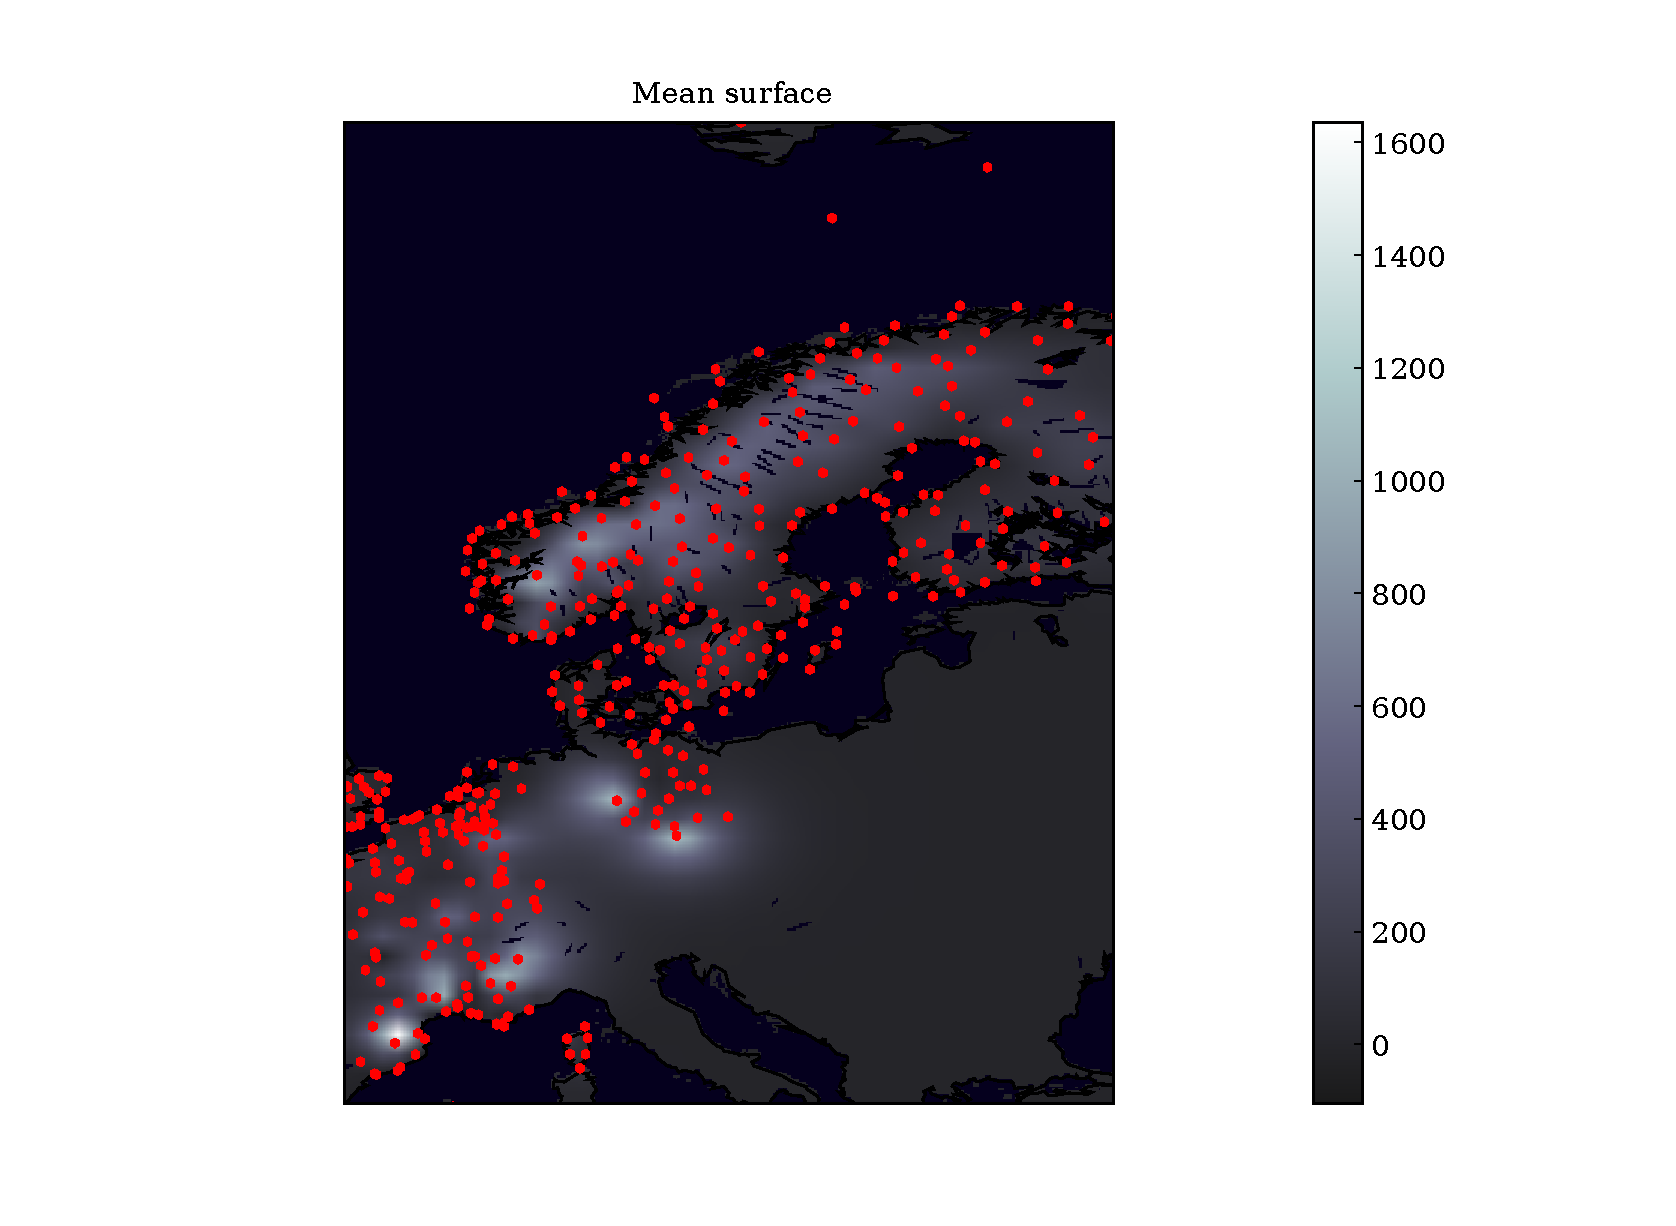
\epsfig{file=figs/elevmean.pdf, width=8cm}
        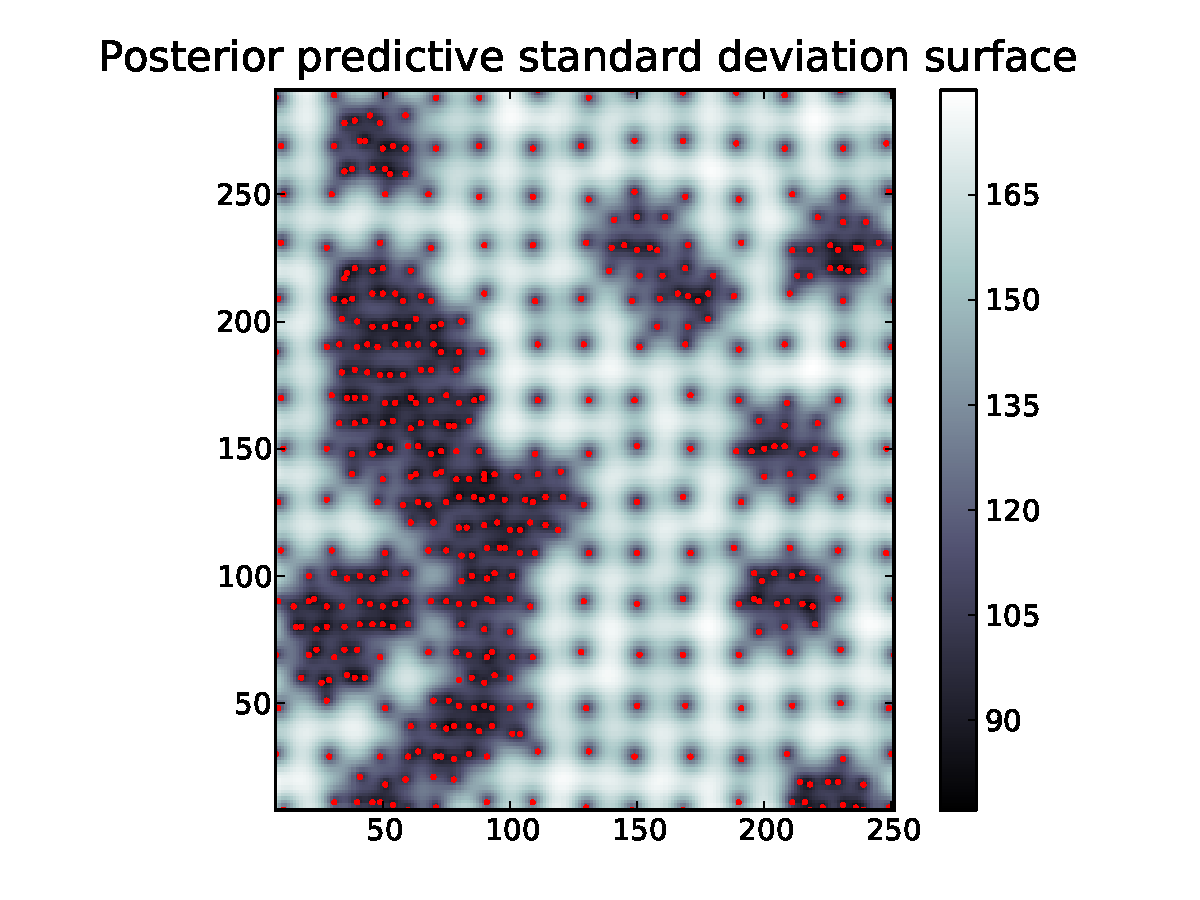
\epsfig{file=figs/elevvar.pdf, width=8cm}
    \caption{The posterior mean and variance surfaces for the $v$ variable of the Walker lake example. The posterior variance is relatively small in the neighborhood of observations, but large in regions where no observations were made.}
    \label{fig:walker}
\end{figure}
\begin{figure}
    \centering
        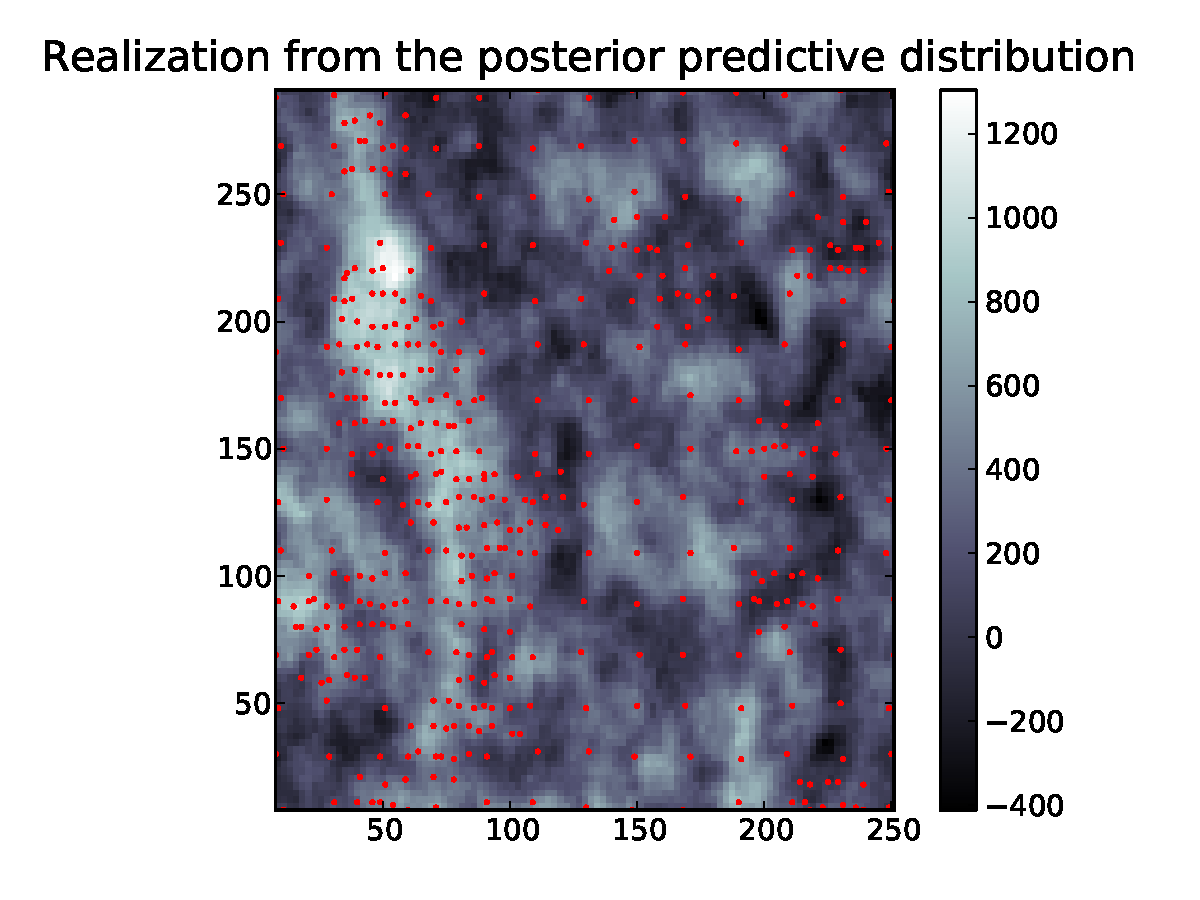
\epsfig{file=figs/elevdraw0.pdf, width=8cm}
        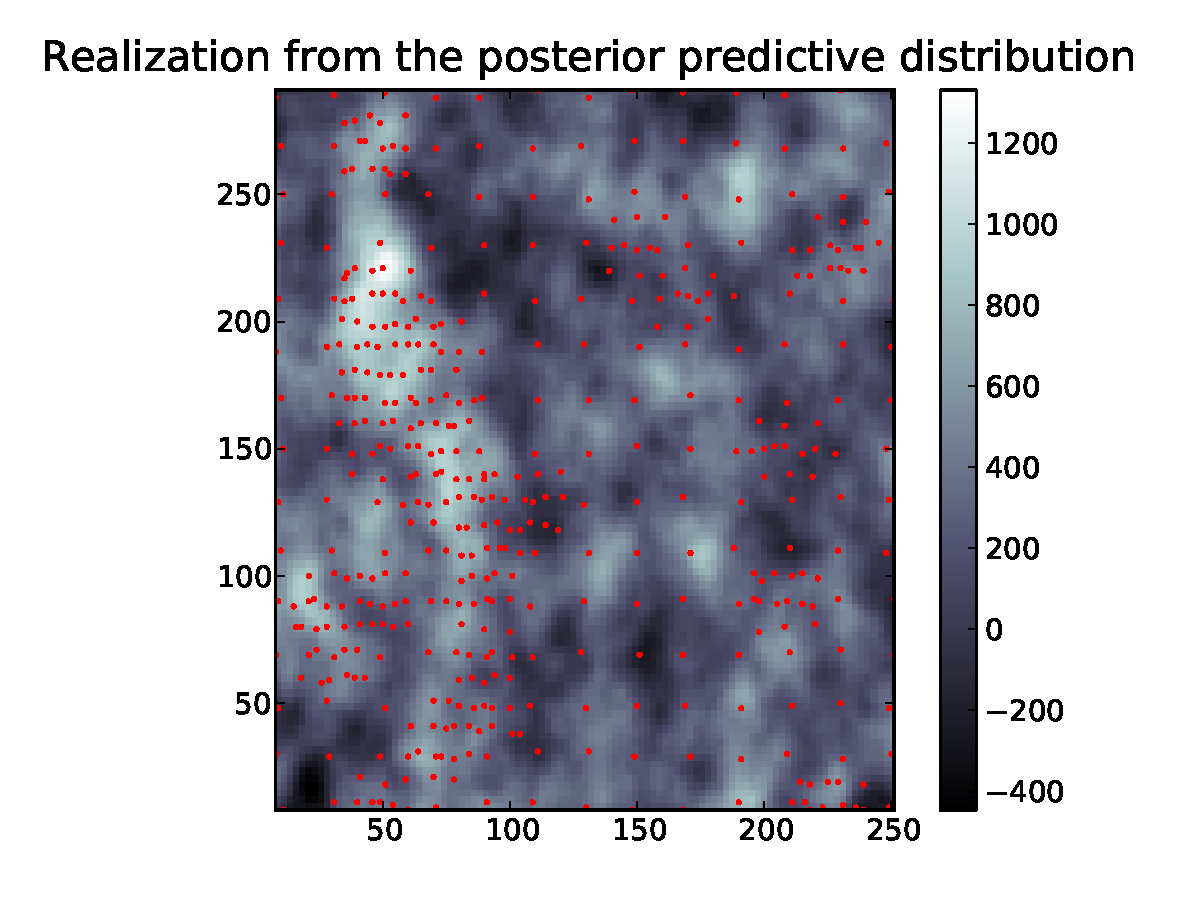
\epsfig{file=figs/elevdraw1.pdf, width=8cm}
    \caption{Two realizations from the posterior distribution of the $v$ surface for the Walker Lake example. Elevation is measured in meters.}
    \label{fig:walkerreal}
\end{figure}
Bayesian geostatistics is demonstrated in the folder \file{examples/gp/more_examples/Geostatistics}. File \file{getdata.py} downloads the Walker Lake dataset of Isaaks and Srivastava \cite{isaaks} from the internet and manipulates the $x$ and $y$ coordinates into the array format described in section \ref{sec:highdim}. File \file{model.py} contains the geostatistical model specification, which is

\begin{eqnarray*}
    d|f \sim \textup{Normal}(f(x),V)\\
    f|M,C \sim \textup{GP}(M,C) \\
    M:x\rightarrow m\\
    C:x,y,\mathtt{amp},\mathtt{scale},\mathtt{diff\_degree}\rightarrow \mathtt{matern.euclidean}(x,y;\mathtt{amp},\mathtt{scale},\mathtt{diff\_degree})\\
    p(m)\propto 1\\
    \mathtt{amp}\sim \textup{Exponential}(7e-5) \\
    \mathtt{scale}\sim \textup{Exponential}(4e-3) \\
    \mathtt{diff\_degree}\sim \textup{Uniform}(.5,2)\\ 
    V\sim \textup{Exponential}(5e-9)\\
\end{eqnarray*}

File \file{mcmc.py} fits the model and produces output maps.  The output of \file{mcmc.py} is shown in figures \ref{fig:walker} and \ref{fig:walkerreal}. Figure \ref{fig:walker} shows the posterior mean and variance of the $v$ variable of the dataset, which is a function of elevation (see Isaaks and Srivastava \cite{isaaks}, appendix A). The mean and variance surfaces are generated conveniently from the trace as follows:
\begin{verbatim}
    Msurf = zeros(dplot.shape[:2])
    E2surf = zeros(dplot.shape[:2])
    for i in xrange(n):
        WalkerSampler.remember(i)
        Msurf_i = WalkerSampler.walker_v.M_obs.value(dplot)
        Msurf += Msurf_i / n
        E2surf += (WalkerSampler.walker_v.C_obs.value(dplot) + Msurf_i**2) / n
\end{verbatim}
The call \texttt{WalkerSampler.remember(i)} resets all the variables in the model to their values at frame $i$ of the MCMC trace. The surfaces $E[v]$ (\texttt{Msurf}) and $E[v^2]$ (\texttt{E2surf}) are easily accumulated by stepping through the trace using \texttt{remember} and evaluating the \texttt{M_obs} and \texttt{C_obs} attributes of the Gaussian process submodel on input array \texttt{dplot}. The standard deviation surface is generated using the standard formula:
\begin{verbatim}
    Vsurf = E2surf - Msurf**2
    SDsurf = sqrt(Vsurf)
\end{verbatim}

Figure \ref{fig:walkerreal} shows two realizations from the posterior predictive distribution of the $v$ surface. They are much rougher than their mean surface, and also much more expensive to compute. However, they are equally convenient to evaluate:
\begin{verbatim}
    indices = random_integers(n,size=2)
    for j,i in enumerate(indices):
        WalkerSampler.remember(i)
        R = WalkerSampler.walker_v.f.value(dplot)
\end{verbatim}
Again, \texttt{remember} is used to reset the model to a randomly-selected frame of the trace, and the Gaussian process $f$ is evaluated on \texttt{dplot} in that frame.






\section{Biological example: Munch, Kottas and Mangel's stock-recruitment study}\label{sub:MMKMCMC}

% \begin{figure}
%     \centering
%     % FIXME: Re-render this graph
%         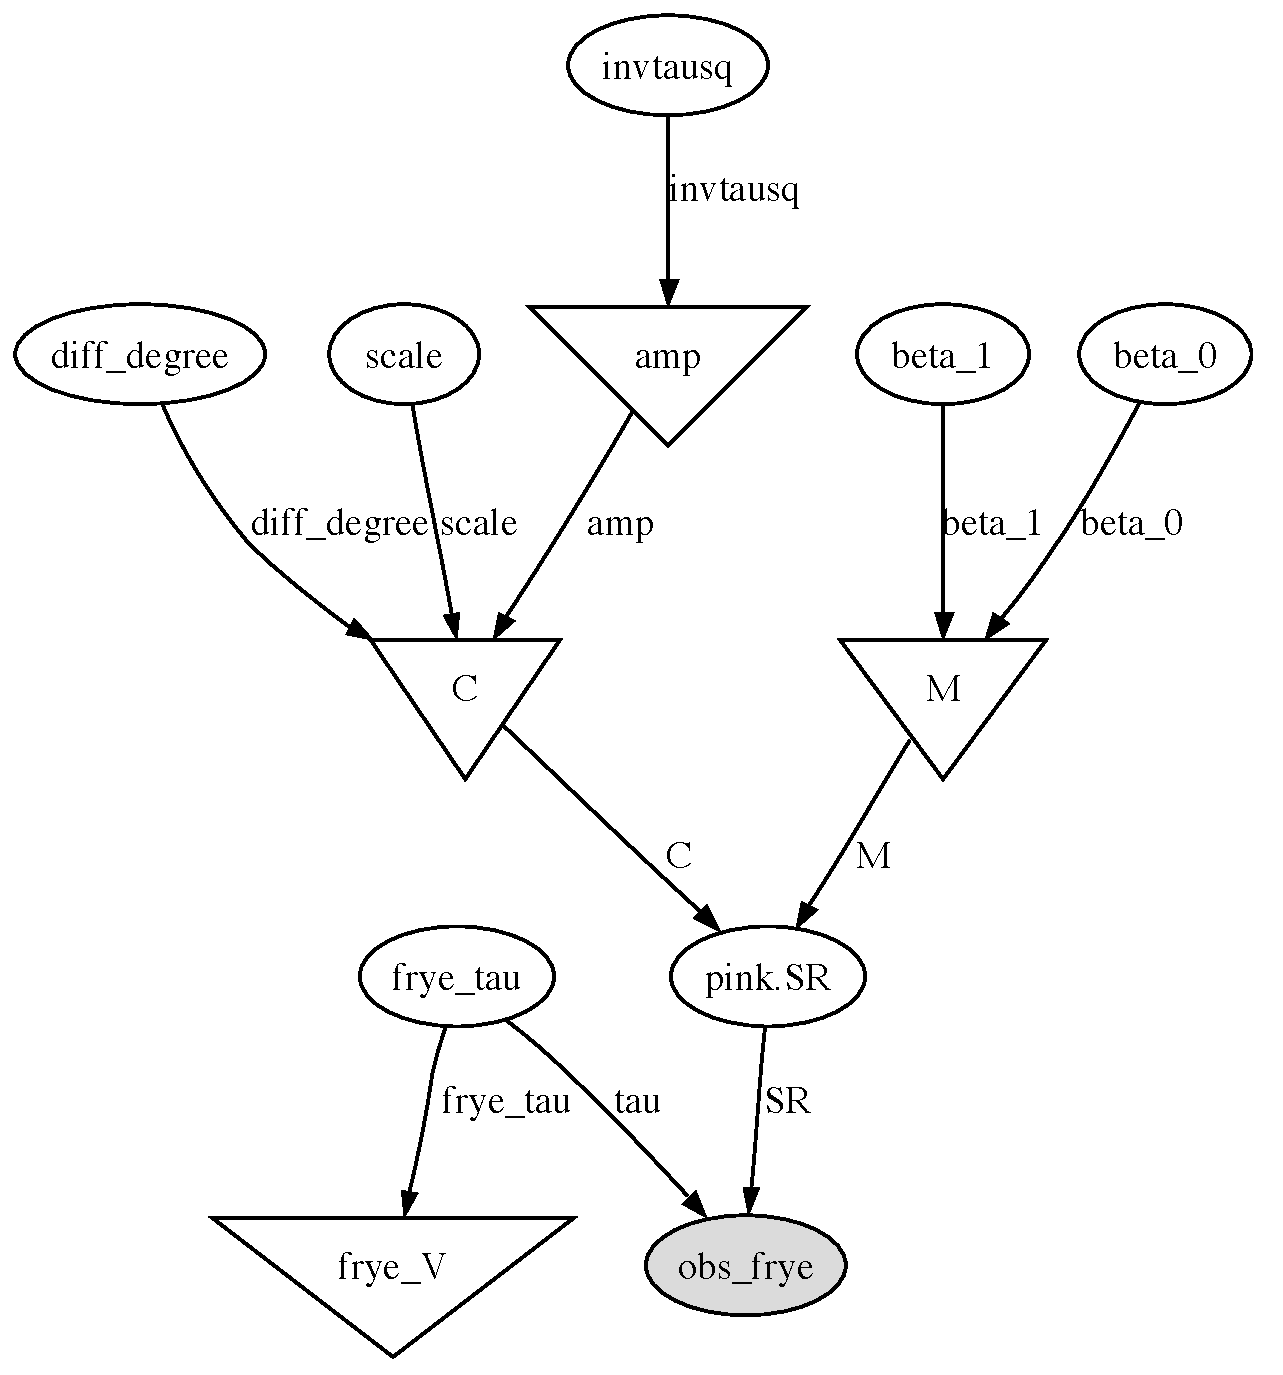
\epsfig{file=figs/MKMsalmon.pdf, width=10cm}
%     \caption{A PyMC-generated directed acyclic graph representation of the probability model in (\ref{eqn:MMKModel}), which is implemented in file \sffamily{`examples/gp/more_examples/MKMSalmon/salmon_sampler.py'}. A very similar probability model was used by Munch, Kottas and Mangel to infer stock-recruitment functions for three salmonid species. The label `\texttt{pink.SR}' indicates that this particular model corresponds to the pink salmon (\emph{Onchorhynchus gorbuscha}) data. Note that two coordinate transformations are implemented using PyMC deterministic variables. This technique can help lazy programmers avoid transforming priors by hand, and in less trivial cases it can save computation by caching the transformed parameters.}
%     \label{fig:MMKsalmonmodel}
% \end{figure}

\begin{figure}
    \centering
        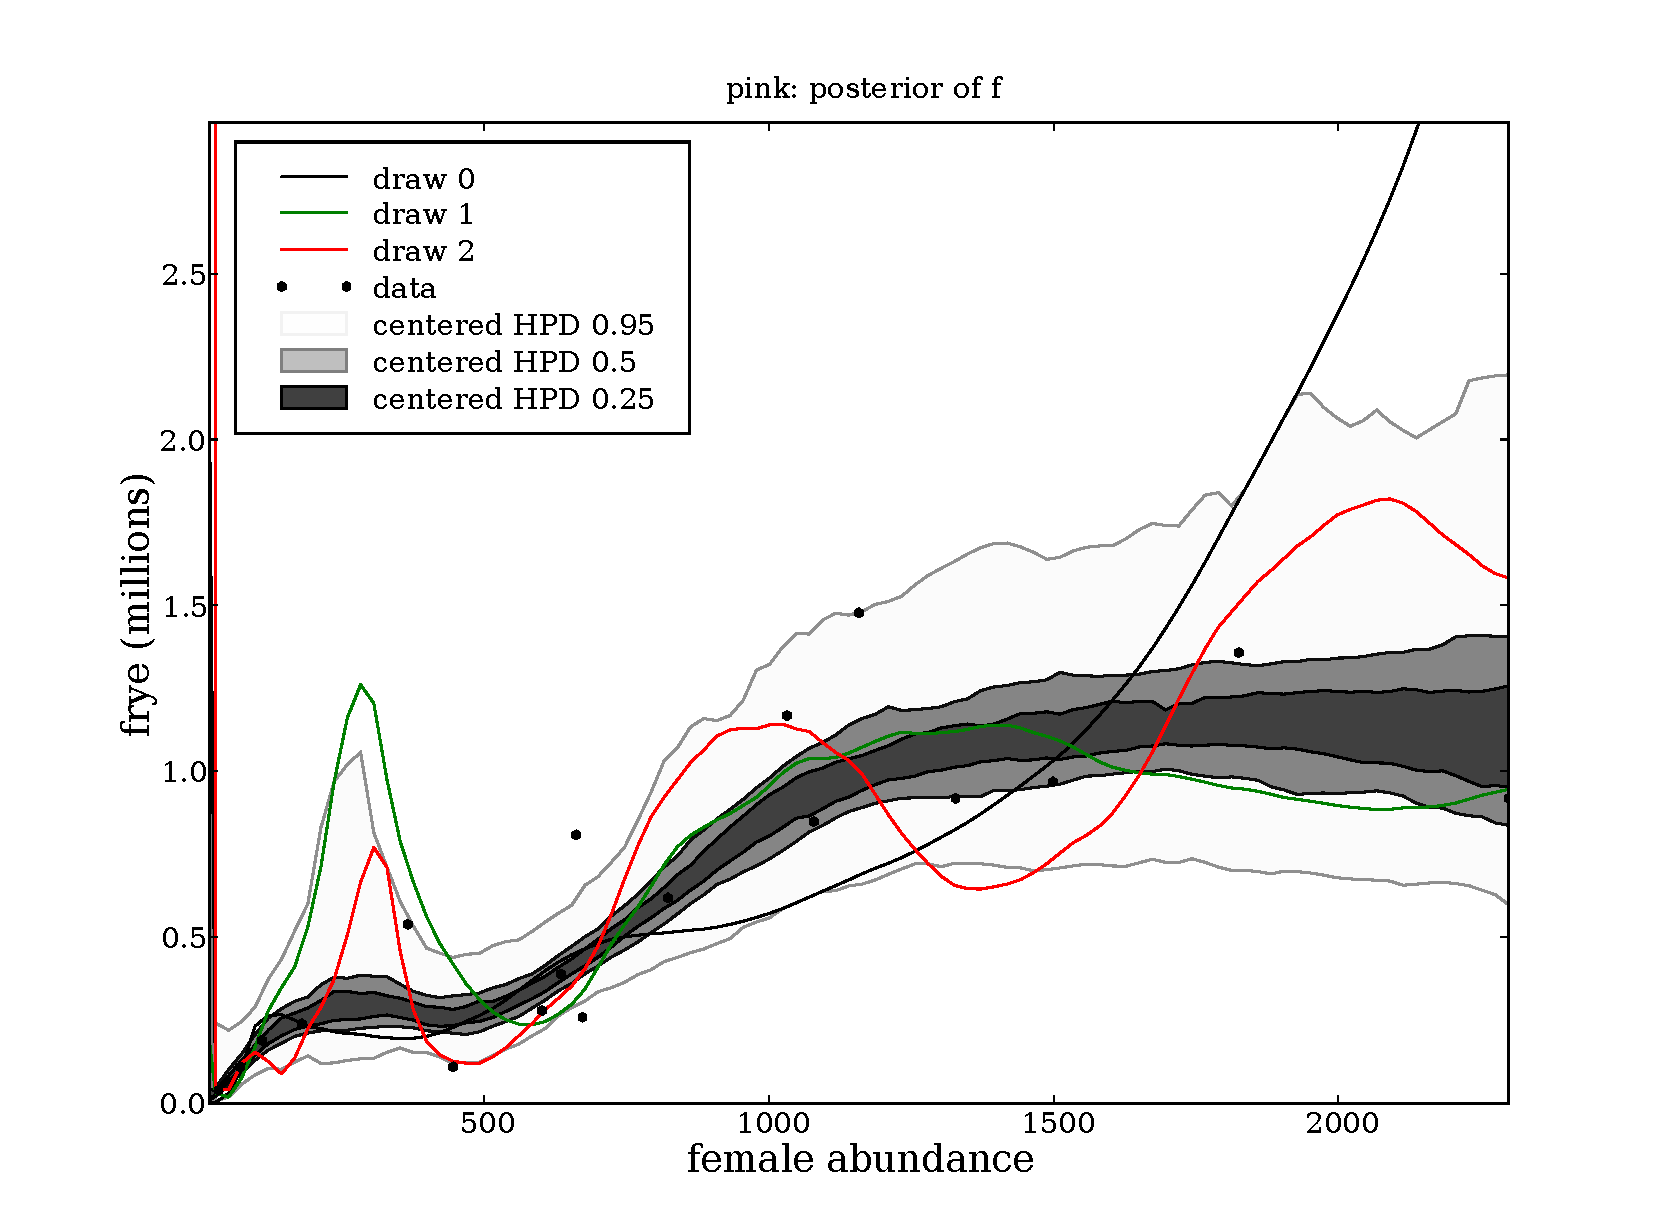
\epsfig{file=figs/pinkfpost.pdf, width=10cm}
    \caption{The posterior of the stock-recruitment function for pink salmon (\emph{Onchorhynchus gorbuscha}). The data are shown as heavy black dots. The centered 95\%, 50\% and 25\% posterior probability intervals are shown as shaded regions. Three draws from the posterior are plotted.}
    \label{fig:pinkfpost}
\end{figure}

\begin{figure}
    \centering
        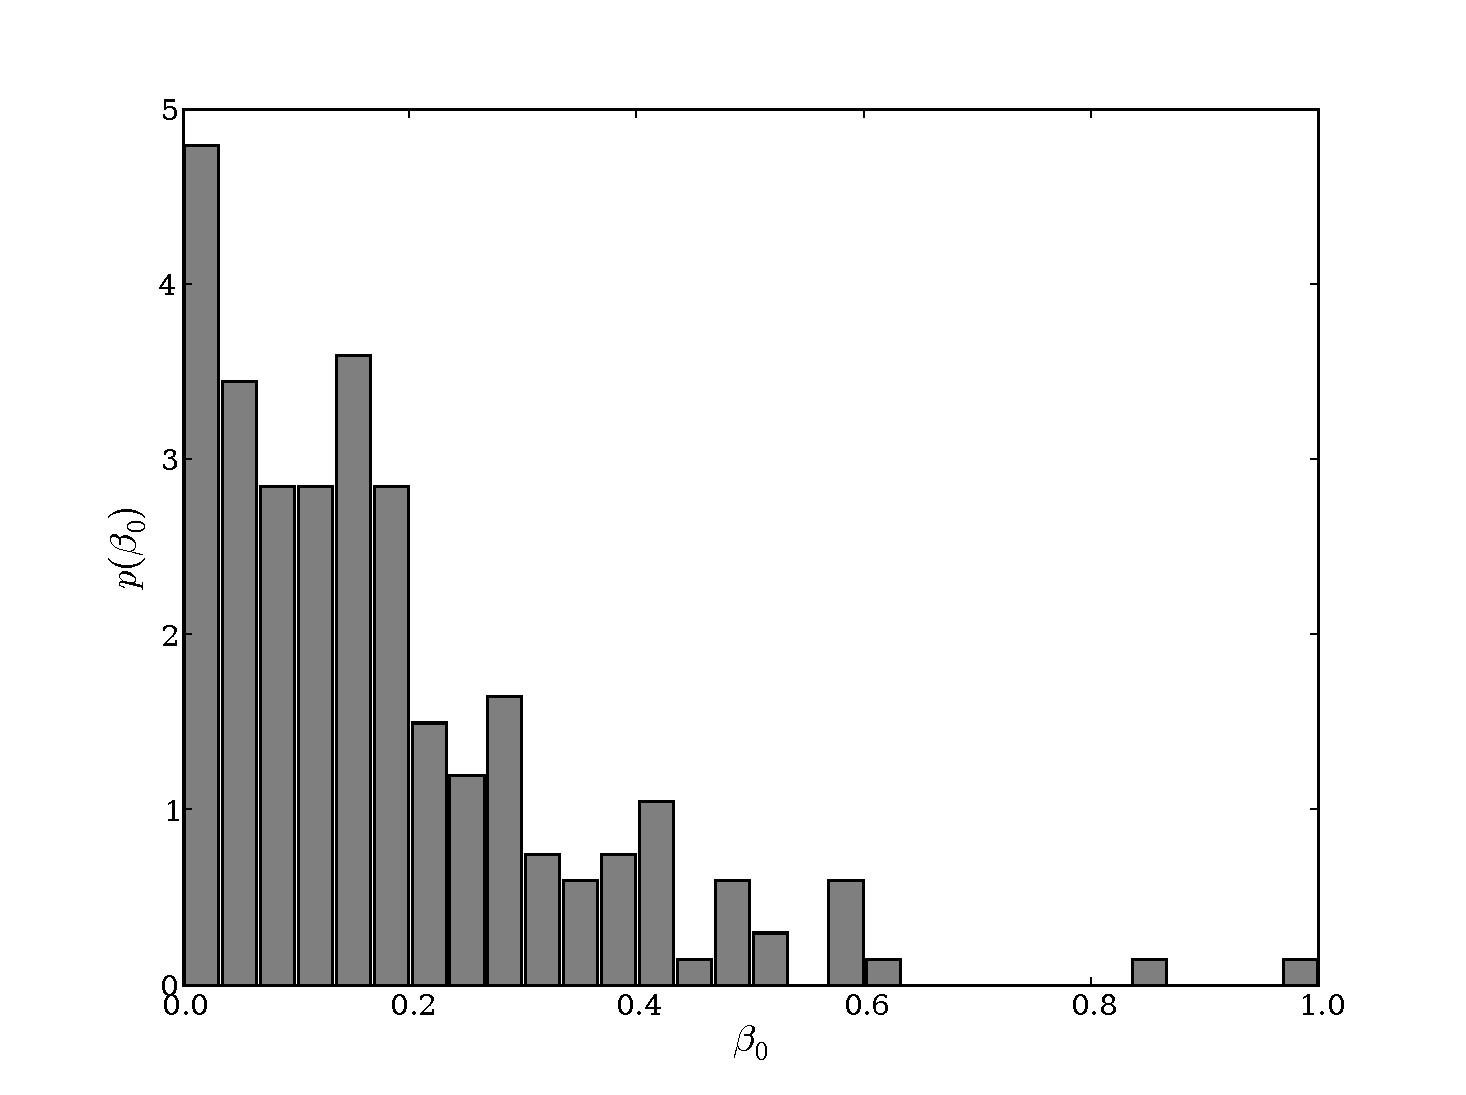
\epsfig{file=figs/pinkbeta0post.pdf, width=5cm}
        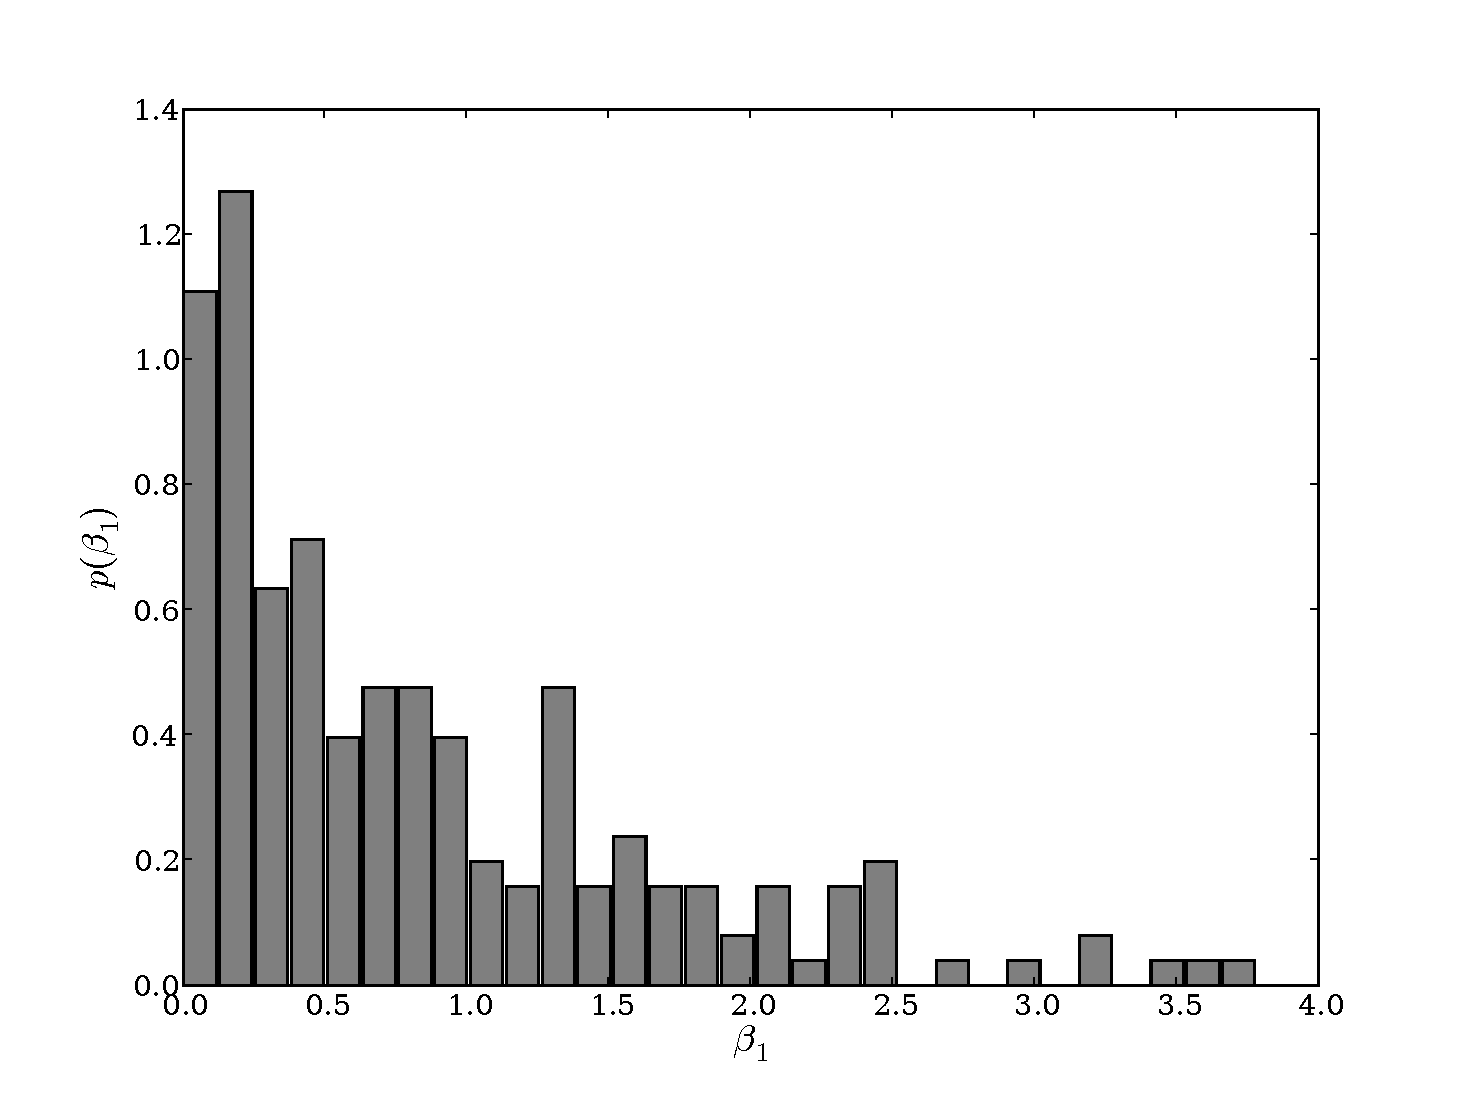
\epsfig{file=figs/pinkbeta1post.pdf, width=5cm}
        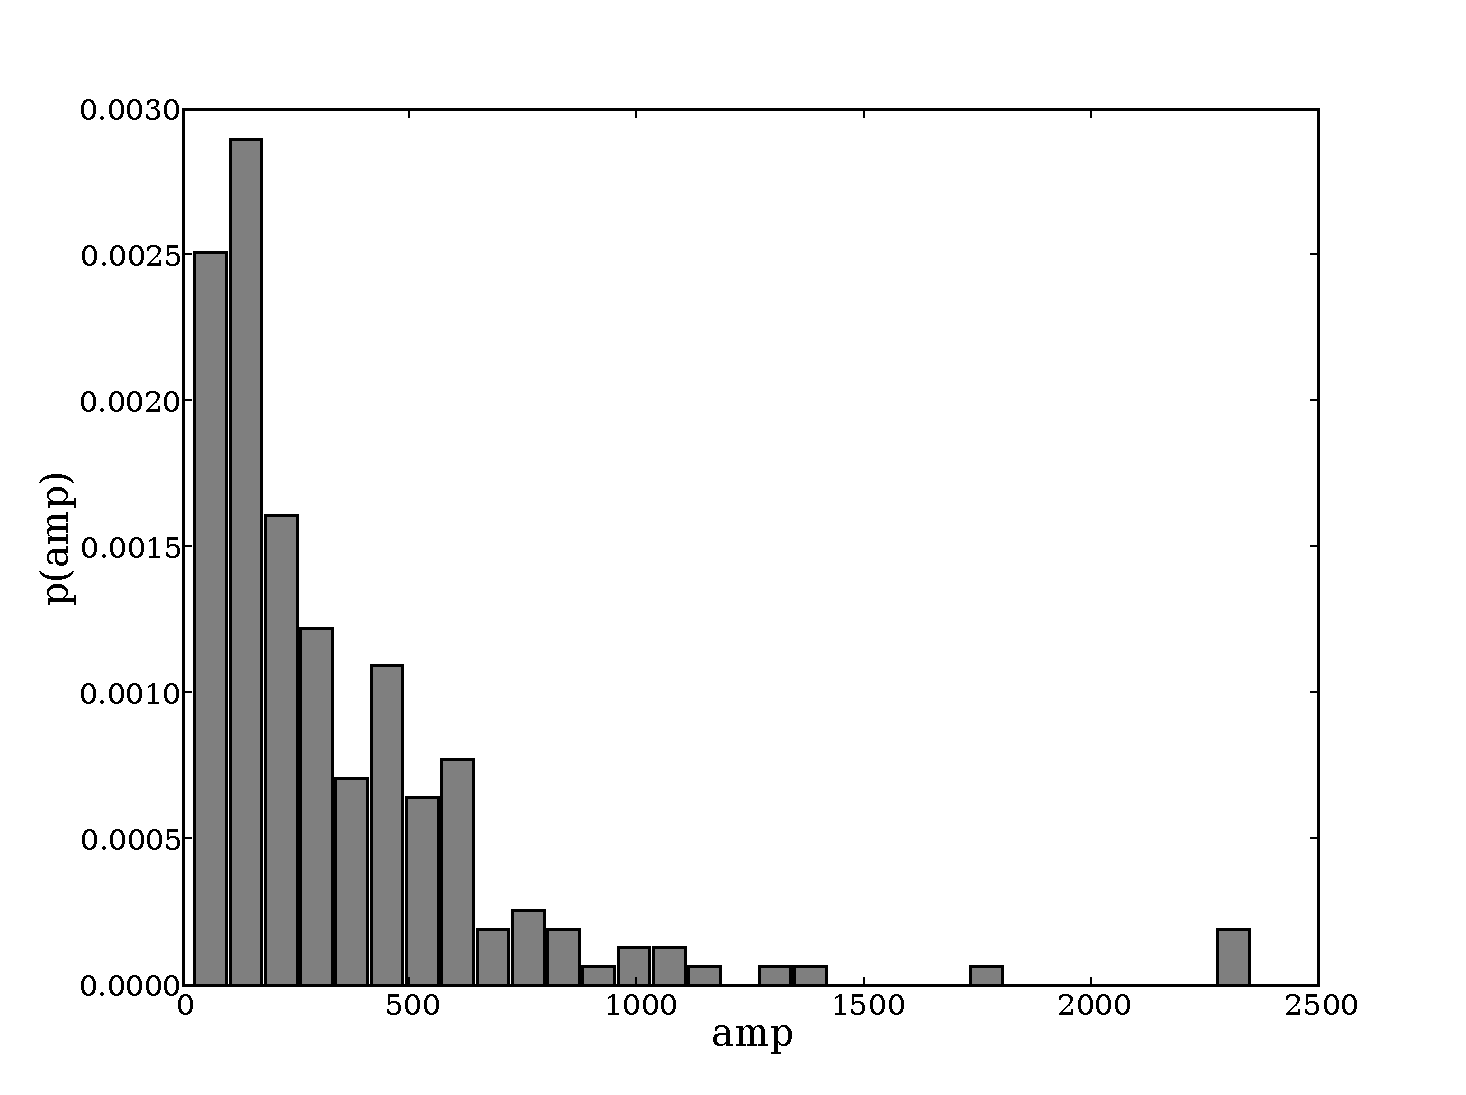
\epsfig{file=figs/pinkamppost.pdf, width=5cm}
        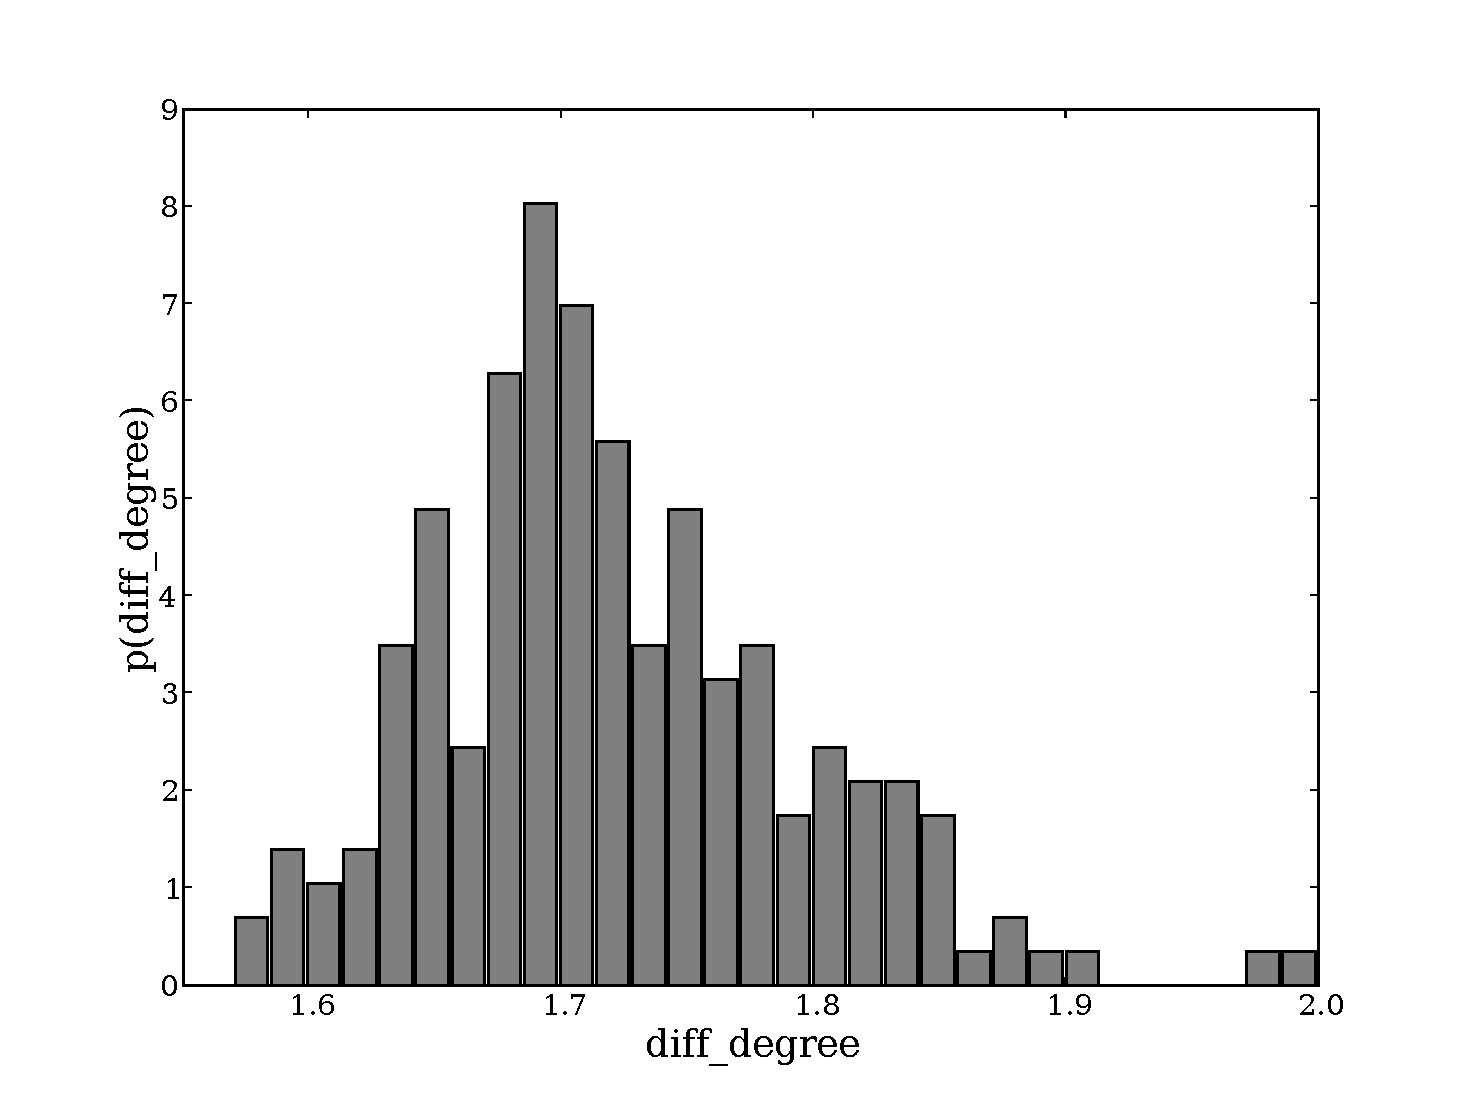
\epsfig{file=figs/pinkdiffdegreepost.pdf, width=5cm}
        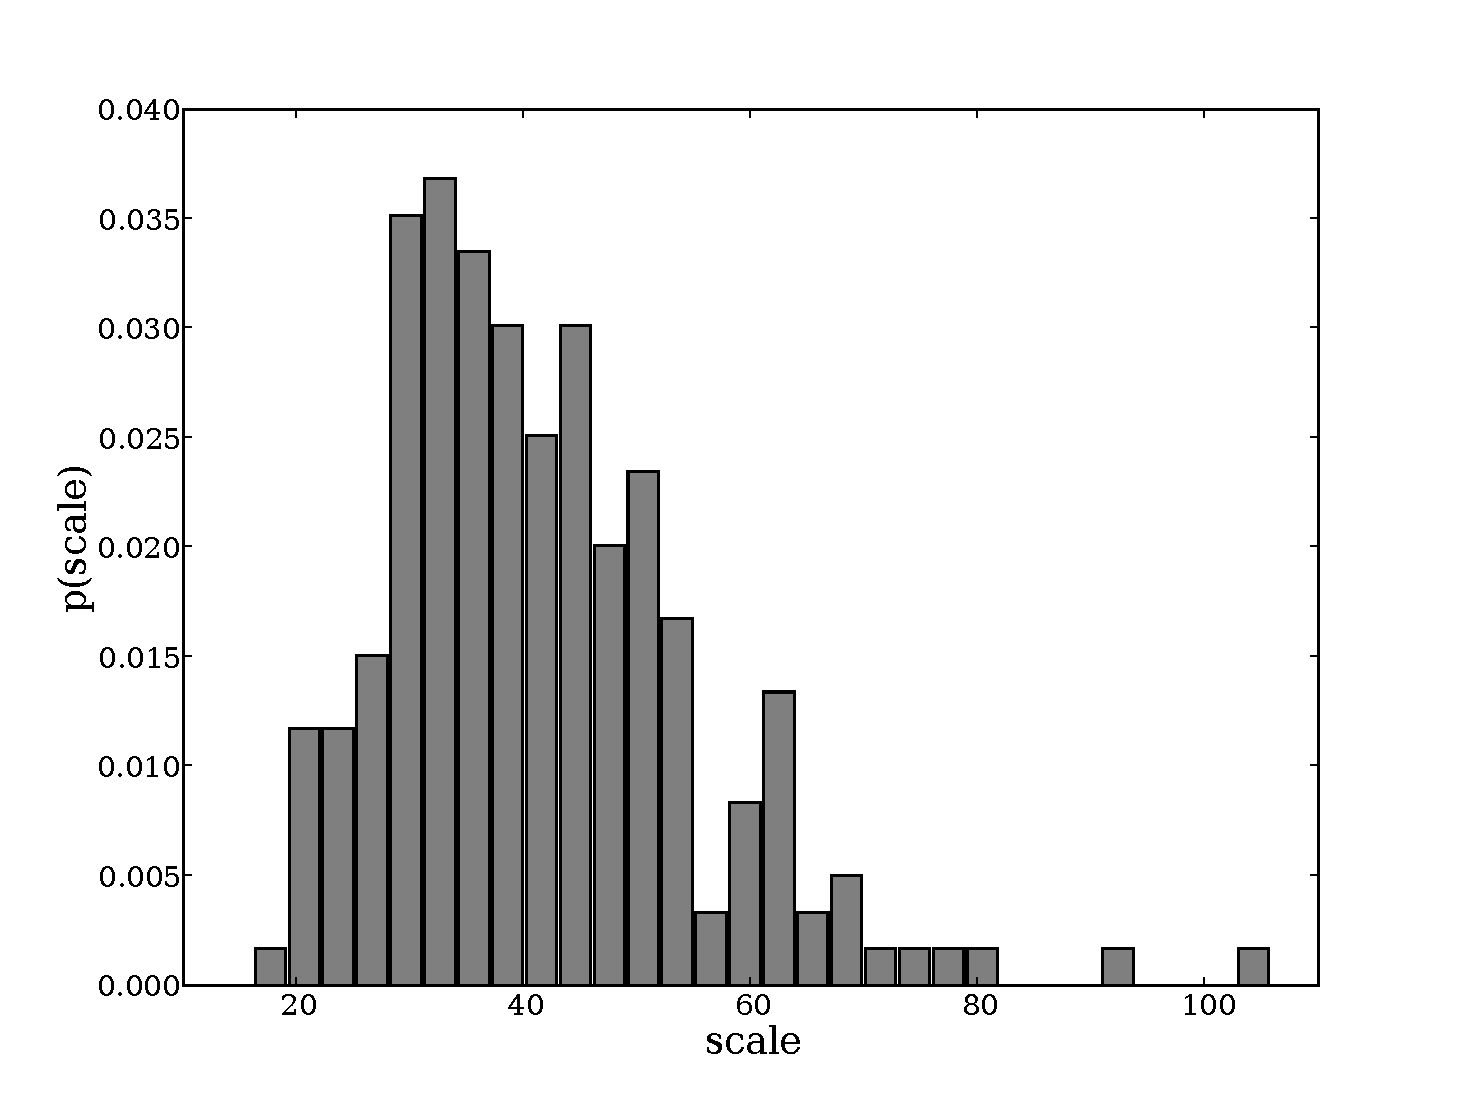
\epsfig{file=figs/pinkscalepost.pdf, width=5cm}
        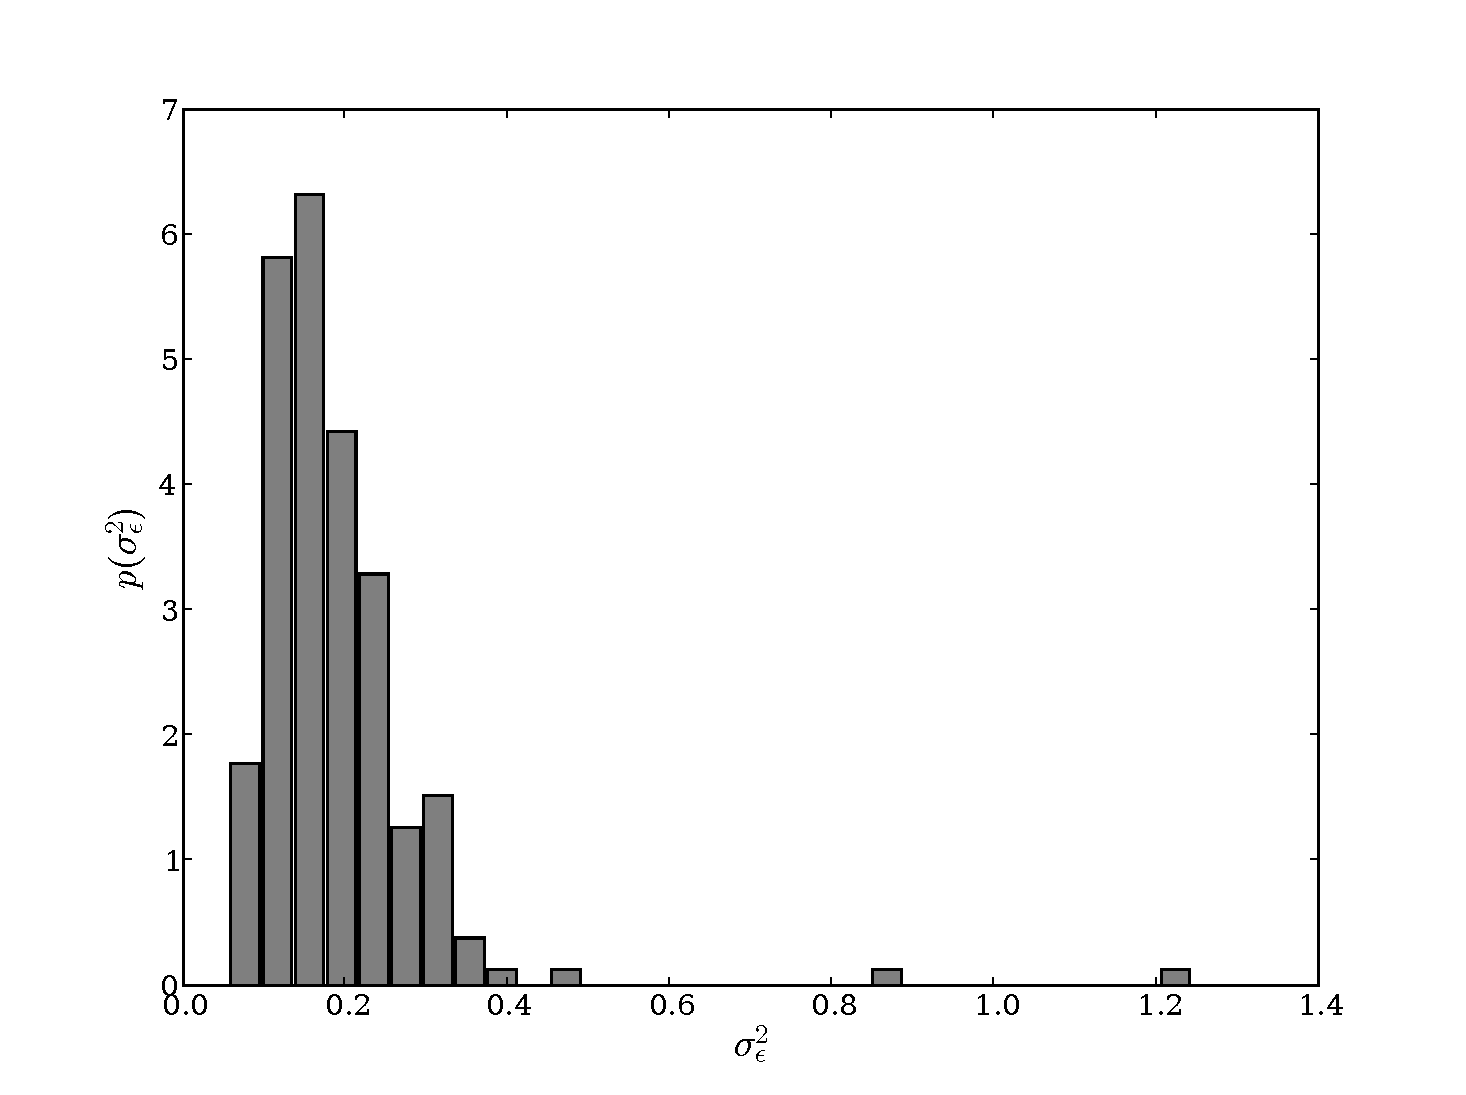
\epsfig{file=figs/pinkVpost.pdf, width=5cm}
    \caption{The marginal posterior distributions of the mean and covariance parameters of the stock-recruitment function for pink salmon (\emph{Onchorhynchus gorbuscha}).}
    \label{fig:pinkparams}
\end{figure}

We now have the tools to duplicate Munch, Kottas and Mangel's \cite{mmk} stock-recruitment results. The full probability we will use follows. It is like Munch, Kottas and Mangel's probability model, but we will use a Mat\`ern covariance function. Here \texttt{SR} is the stock-recruitment function, C is its covariance and M is its mean.
\begin{equation}
    \label{eqn:MMKModel}
    \begin{array}{ll}
        \texttt{frye}[i] \stackrel{\tiny{\textup{ind}}}{\sim} \textup{N}(exp(\mathtt{SR}(\log(\mathtt{abundance}[i]))), V),& i=1\ldots n\\
        \texttt{SR}\sim \textup{GP}(M,C)& \\
        M:x\rightarrow \beta_0+\beta_1 \log(x)&\\
        C:x,y\rightarrow \texttt{matern.euclidean}(x,y;\ \texttt{diff_degree},\texttt{amp},\texttt{scale})&\\
        V,\ \beta_0,\ \beta_1,\ \texttt{diff_degree},\ \texttt{amp},\ \texttt{scale} \sim \texttt{priors}.&
    \end{array}
\end{equation}
The priors can be found by reading their paper (except the prior on \texttt{diff_degree}, which I chose) or by reading the file \file{examples/more_examples/MMKSalmon/salmon_sampler.py}. This file contains a PyMC \texttt{MCMC} subclass called \texttt{SalmonSampler}, which reads in the data, creates a probability model incorporating the data, and provides some plotting methods.

Note that this model differs from the model in section \ref{sub:MMKregression} in that we're putting a Gaussian process prior on the stock-recruitment function in log-log space, so conditioning its value at zero is not an option.

% The probability model \texttt{SalmonSampler} creates is visualized as a directed acyclic graph in figure \ref{fig:MMKsalmonmodel}. 

Munch, Kottas and Mangel specify priors for $\texttt{amp}^{-2}$ and $V^{-1}$, and we have used PyMC deterministic variables to conveniently implement the transformations rather than changing variables manually. The posterior distribution of \texttt{SR} for the pink salmon (\emph{Onchorhynchus gorbuscha}) is shown in figure \ref{fig:pinkfpost}, and the posterior of the mean and covariance parameters for the same species are shown in figure \ref{fig:pinkparams}.




% \chapter{Old stuff} 
% 
% \section{The \texttt{GP} class}
% \texttt{GP} is a subclass of the PyMC \texttt{Stochastic} class whose value attribute is a \texttt{Realization} instance. Its init method takes the following arguments:
% \begin{description}
%     \item[$M$:] A mean object or mean-valued deterministic variable.
%     \item[$C$:] A covariance object or covariance-valued deterministic variable.
%     \item[\texttt{mesh=None}:] An array or an array-valued variable.
%     \item[\texttt{init_mesh_vals=None}:] An optional vector of initial values for the value attribute's evaluation on \texttt{mesh}.
%     \item[\texttt{mesh_eval_isdata=False}:] If \texttt{True}, the value attribute's evaluation on \texttt{mesh} is fixed at \texttt{init_mesh_vals}.
%     \item[\texttt{doc, name, trace, cache_depth, verbose}:] Optional arguments that are passed directly to \code{Stochastic.\_\_init\_\_}. See PyMC's documentation.
% \end{description}
% 
% \texttt{GP} instances have a log-probability attribute like any PyMC stochastic variable, but there is an important difference: If the value attribute is a realization called $f$, the log-probability attribute gives $p(f\texttt{(mesh))}|M,C)$. In other words, the log-probability attribute only cares about $f$'s evaluation on \texttt{mesh}. The reason is simple: it would be expensive and difficult to assign something like a log-density to entire realizations in most cases.
% 
% \section{The \texttt{GPMetropolis} and \texttt{GPParentMetropolis} step methods}
% 
% \section{GPMetropolis}
% The Metropolis-Hastings acceptance ratio for a proposed value $f_p$ can be written as follows:
% \begin{eqnarray*}
%     \frac{p(K|\tilde f_p, f_p(\mathtt{mesh}))\ p(\tilde f_p|f_p(\mathtt{mesh}), P)\ p(f_p(\mathtt{mesh}) | P)\ q(\tilde f|f(\mathtt{mesh}))\ q(f(\mathtt{mesh}))}{p(\mathtt{K}|\tilde f, f(\mathtt{mesh}))\ p(\tilde f|f(\mathtt{mesh}), P)\ p(f(\mathtt{mesh}) | P)\ q(\tilde f_p|f(\mathtt{mesh}))\ q(f_p(\mathtt{mesh}))},
% \end{eqnarray*}
% 
% \texttt{GPMetropolis} reports its competence to handle \texttt{GP} instances as \texttt{3}, so it will be chosen as the default handler. Its init method takes the following arguments:
% \begin{description}
%     \item[\texttt{stoch}:] The \texttt{GPMetropolis} instance to be handled.
%     \item[\texttt{scale=.1}:] $f(\texttt{mesh})$ will be proposed from a random-walk multivariate normal distribution with covariance equal to \texttt{C(mesh, mesh * scale * adaptive_scale_factor)}, where C is the covariance-valued parent and \texttt{adaptive_scale_factor} is the adaptive scaling factor, which is updated when \texttt{self.tune()} is called.
%     \item[\texttt{verbose = 0}:] An integer from 0 to 3 indicating the preferred verbosity level.
% \end{description}

% \section{The \texttt{GPNormal} step method}
% As we've already seen in other contexts, a \texttt{GP}'s full conditional distribution is a Gaussian process if its Markov blanket is described by the following probability model:
% \begin{eqnarray*}
%     K_i |f \sim \textup{N}(f(o_i), V_i) & i=0\ldots n-1\\
%     f|M,C\sim\textup{GP}(M,C)
% \end{eqnarray*}
% In other words, each of its children $K_i$ is normally distributed with variance $V_i$ and mean equal to $f(o_i)$, where $o_i$ is an arbitrary mesh.
% 
% In this case, a \texttt{GP} instance $f$ can be handled by the Gibbs step method \texttt{GPNormal}, which will have much better mixing properties that \texttt{GPMetropolis}. Its init method takes the following parameters:
% \begin{description}
%     \item[$f$:] The \texttt{GP} instance to be handled.
%     \item[\texttt{obs_mesh:}] An array or array-valued variable giving the observation mesh $o$.
%     \item[\texttt{obs_V}:] An array or array-valued variable giving the observation variance $V$.
%     \item[\texttt{obs_vals}:] An array or array-valued variable giving the concatenation of the values of the children $K_i$.
% \end{description}
% 
% \texttt{GPNormal} doesn't register itself, so it will never be assigned as a default handler. This may change eventually.
% 
% \texttt{GPNormal} doesn't care about $f$'s mesh, because it never has to evaluate $f$'s log-probability. However, a good choice of mesh is important because it will used by the \texttt{GPParentMetropolis} instances that handle $f$'s mean and covariance parameters.
% 
% 
% % \section{Example: Ellner, Seifu and Smith's blowfly study}\label{sub:ESSMCMC}
% %
% % \textbf{I haven't been able to get this one to mix yet.} The model is:
% % \begin{eqnarray*}
% %     \textup{data}_t \stackrel{\tiny{\textup{ind}}}{\sim}(A_t, V)\\
% %     A_t = B(A_{t-\tau})\psi_{t-\tau} - D(A_{t-1})\phi_{t-1}, & t>\tau\\
% %     B \sim \textup{GP}(sx\exp(-rx), C_B) \\
% %     D \sim \textup{GP}(mx, C_D) \\
% %     \psi_t \stackrel{\tiny{\textup{iid}}}{\sim}\textup{lognorm}(\mu_\phi,V_\phi) \\
% %     \phi_t \stackrel{\tiny{\textup{iid}}}{\sim}\textup{lognorm}(\mu_\phi,V_\phi)\\
% %     C_B = \textup{Mat\`ern}(\sigma_B,\nu_B,\phi_B) \\
% %     C_D = \textup{Mat\`ern}(\sigma_D,\nu_D,\phi_D)   \\
% %     A_{1\ldots\tau},r,s,m,\textup{covariance parameters},\mu_\phi,\mu_\psi,V_\phi,V_\psi,V \sim \textup{priors},
% % \end{eqnarray*}
% % and I assumed $\tau$ fixed for purposes of the demo. The DAG schematic is shown in figure \ref{fig:ESSblowflymodel}.
% %
% % What happens is the following: when $B$ and $D$ have mean zero, the model burns in and mixes badly. When they have the mean functions parametrized above, the amplitude of their covariance params get very small; the model is preferring the simpler parametric version, since it can explain the data as well as the nonparametric version. This would make a great demo for both the importance of a flexible mean function and the natural parsimony of Bayesian statistics, but I can't even get the parametric version mixing and don't have time for week-long runs. We'll see what happens with this.
% %
% % \begin{figure}
% %     \centering
% %         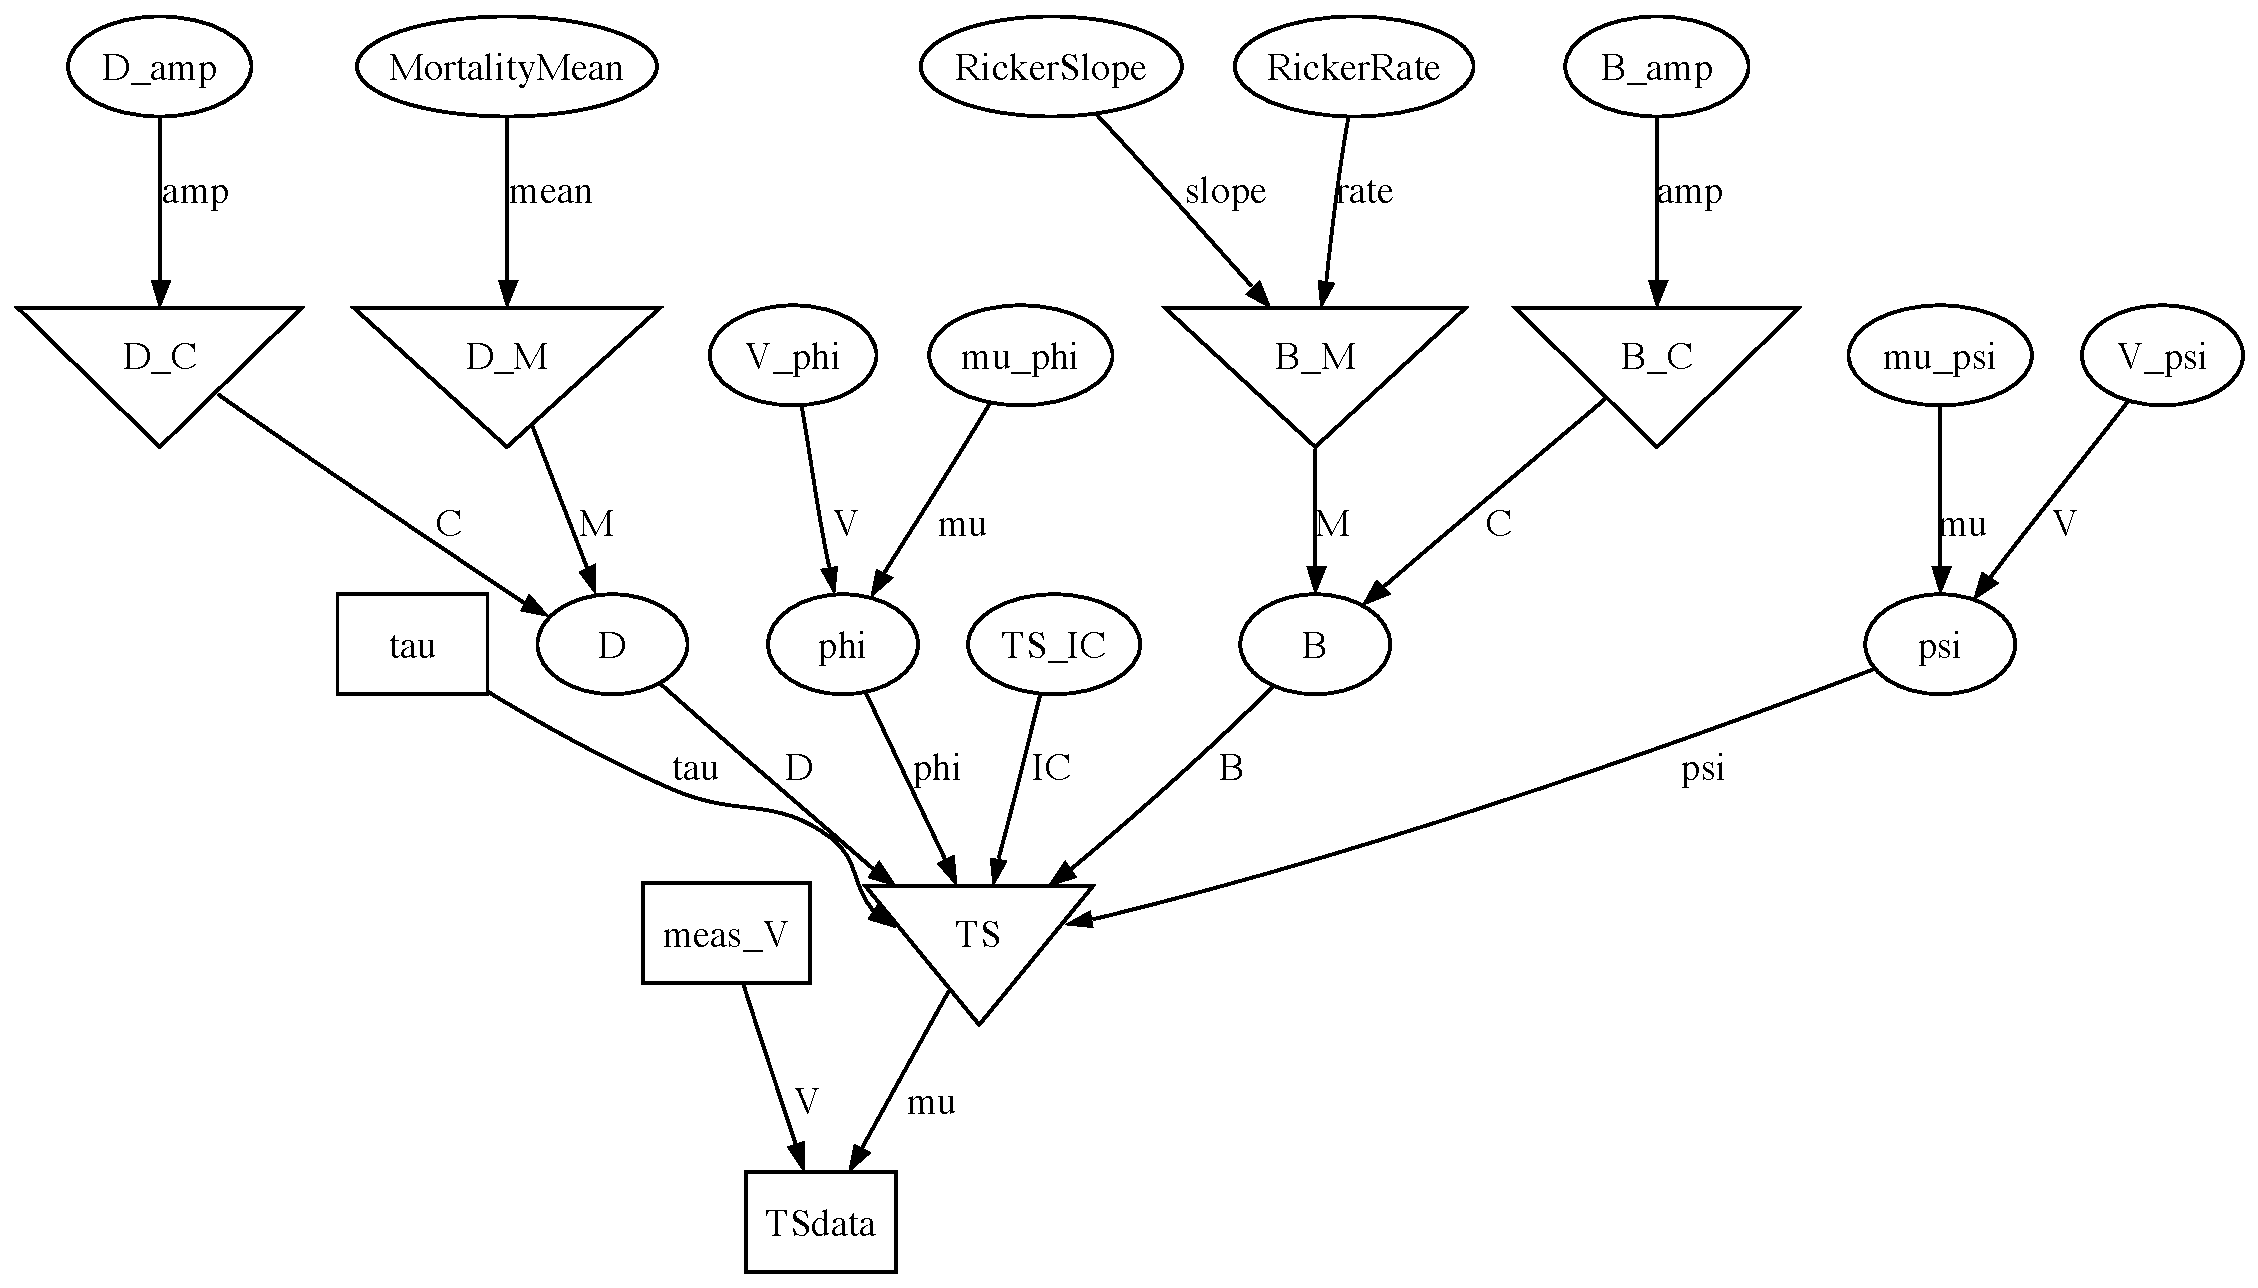
\epsfig{file=figs/ESSblowfly.pdf,width=15cm}
% %     \caption{The model for Ellner, Seifu and Smith's \cite{ess} blowfly data.}
% %     \label{fig:ESSblowflymodel}
% % \end{figure}
% %
% % % \begin{figure}
% % %     \centering
% % %         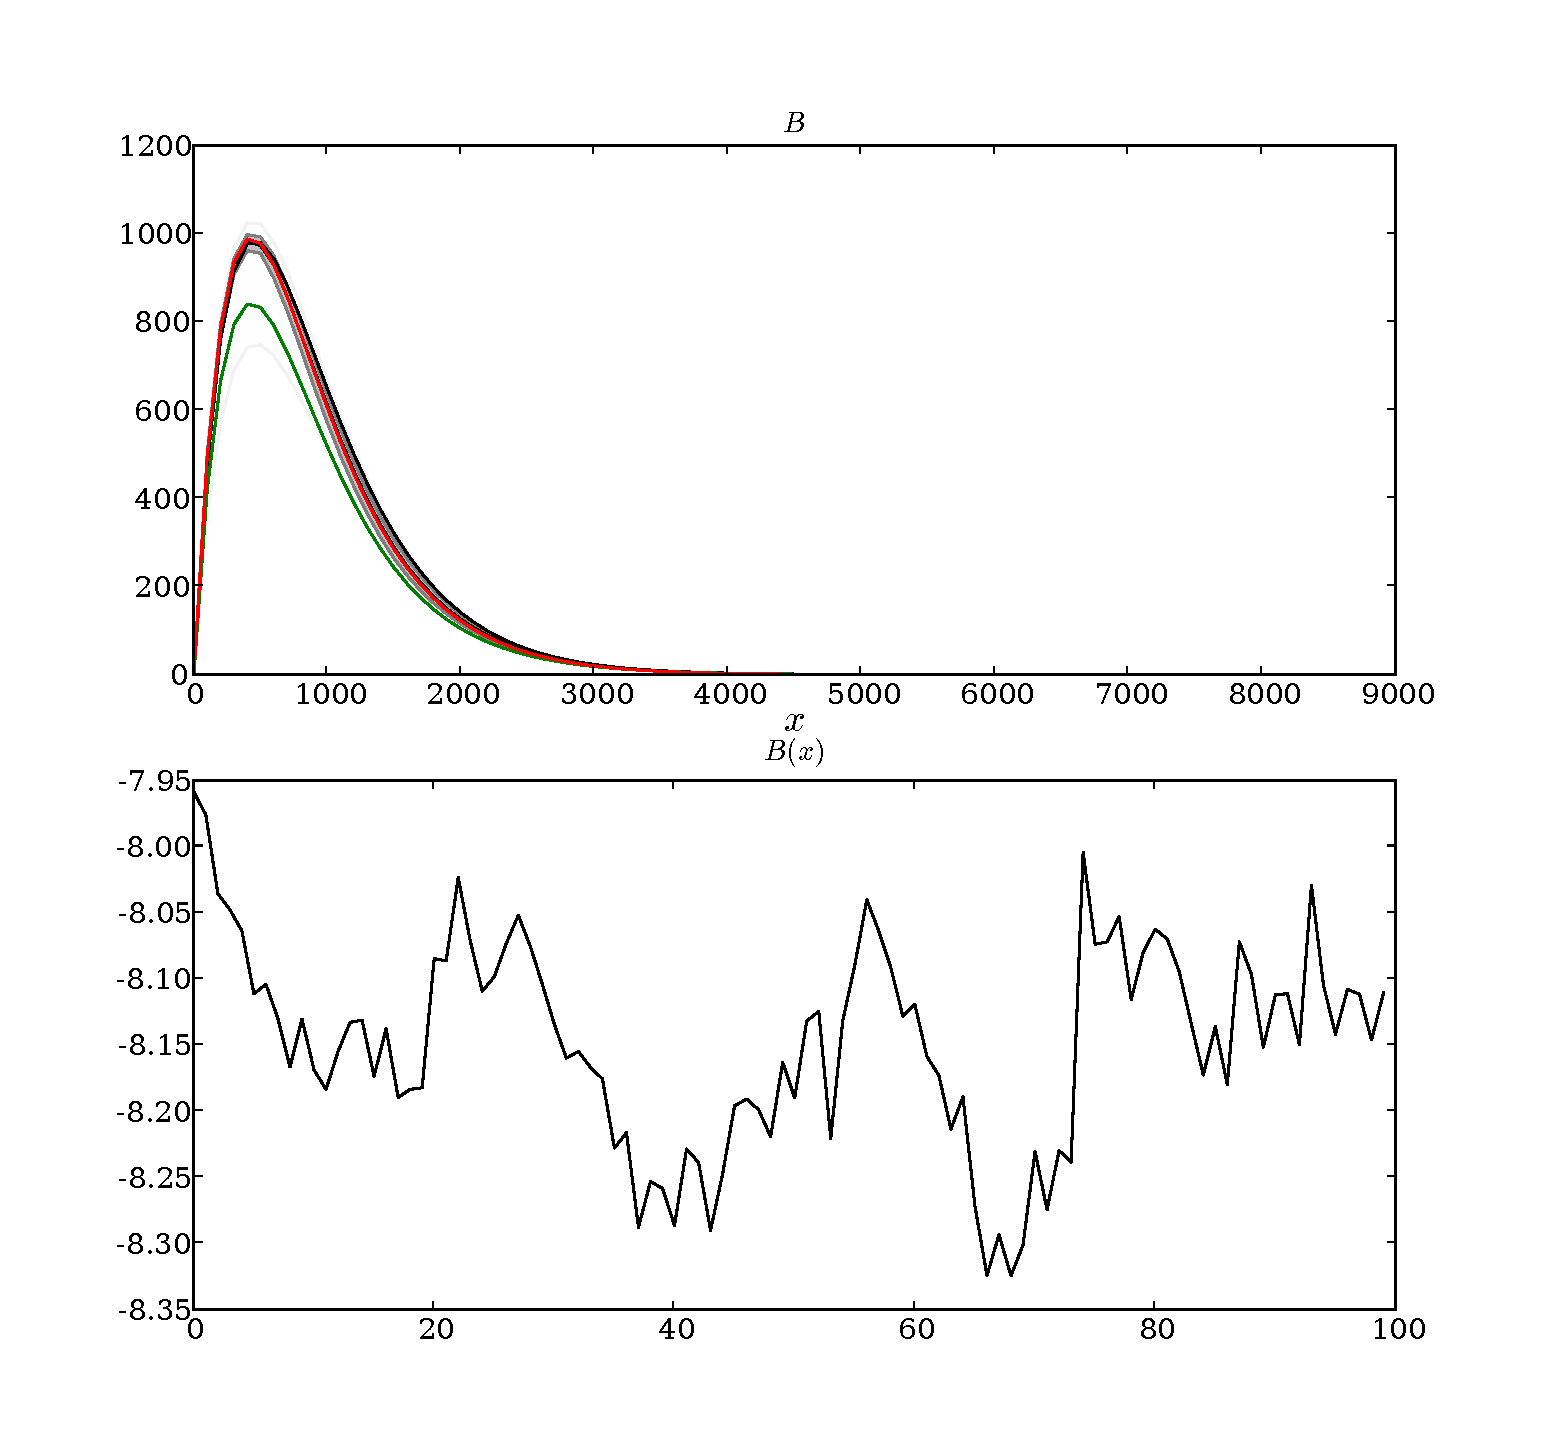
\epsfig{file=figs/ESSBPosterior.pdf,width=10cm}
% % %         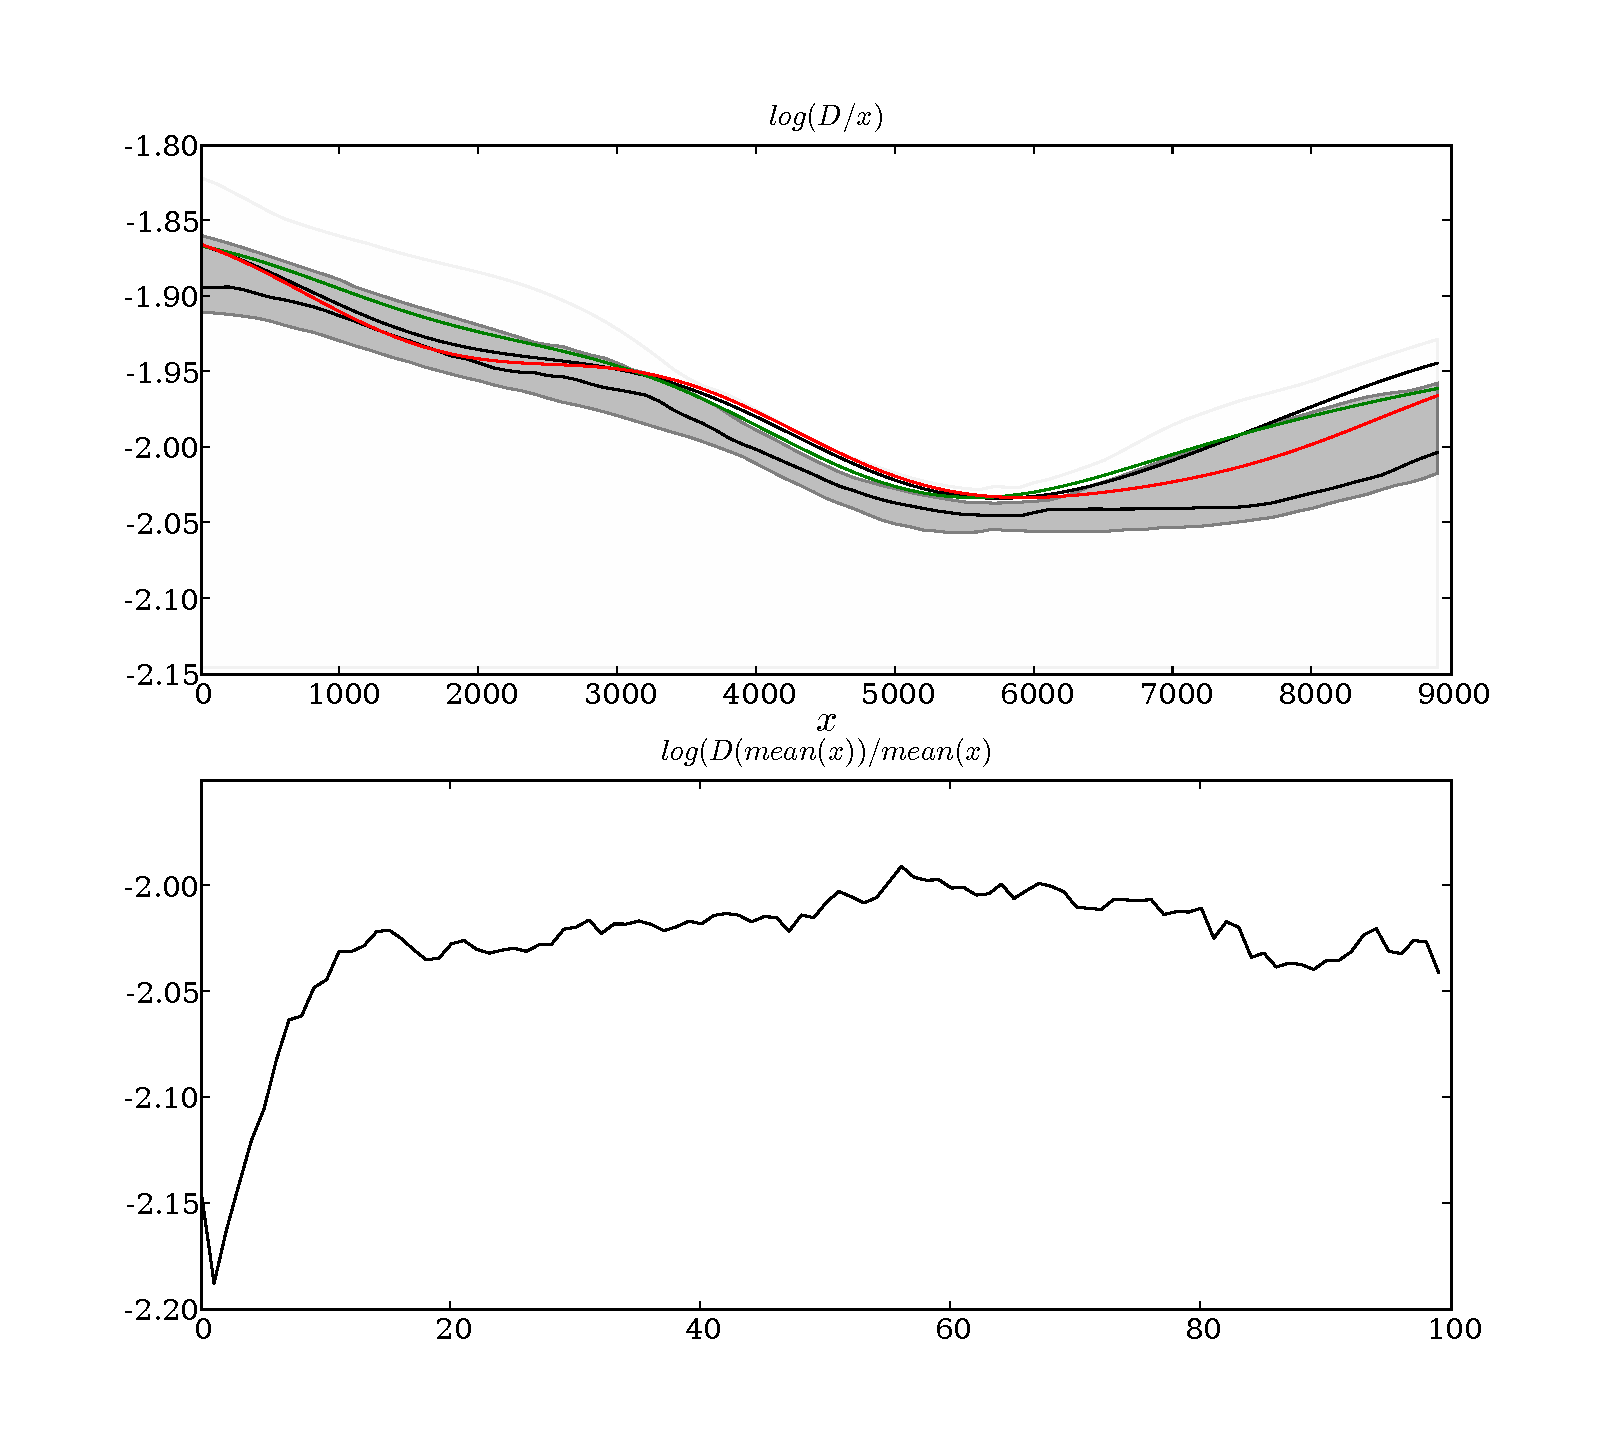
\epsfig{file=figs/ESSDPosterior.pdf,width=10cm}
% % %     \caption{caption}
% % %     \label{fig:ESSBD}
% % % \end{figure}
% % %
% % % \begin{figure}
% % %     \centering
% % %         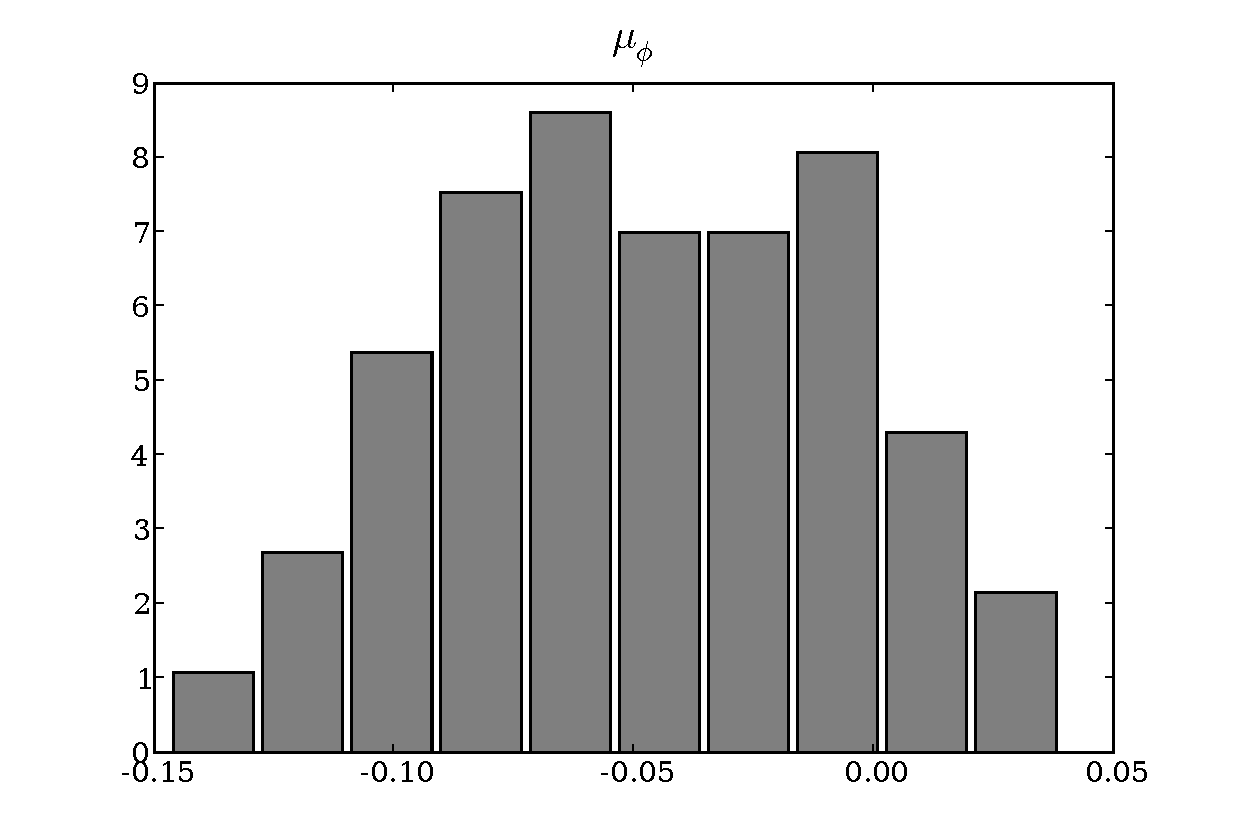
\epsfig{file=figs/ESSmuphiPosterior.pdf,width=7cm}
% % %         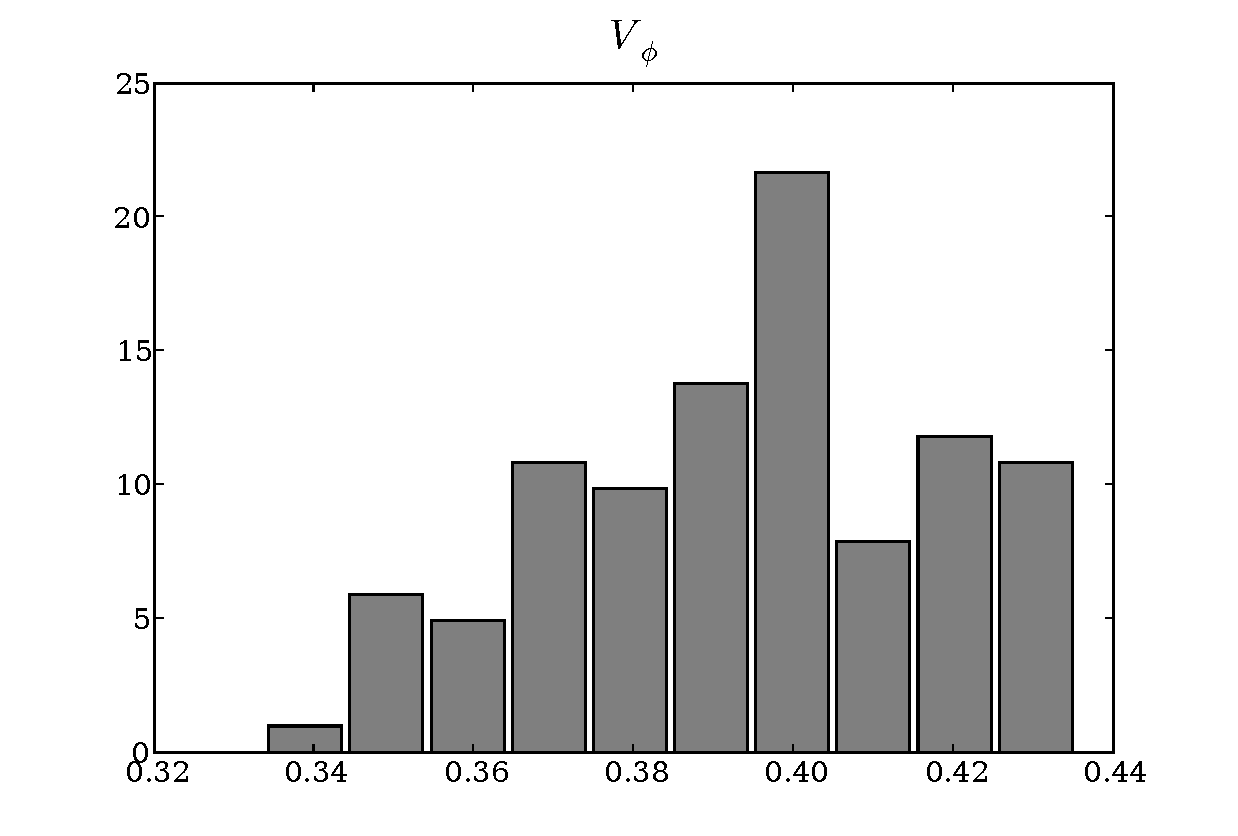
\epsfig{file=figs/ESSVphiPosterior.pdf,width=7cm}
% % %         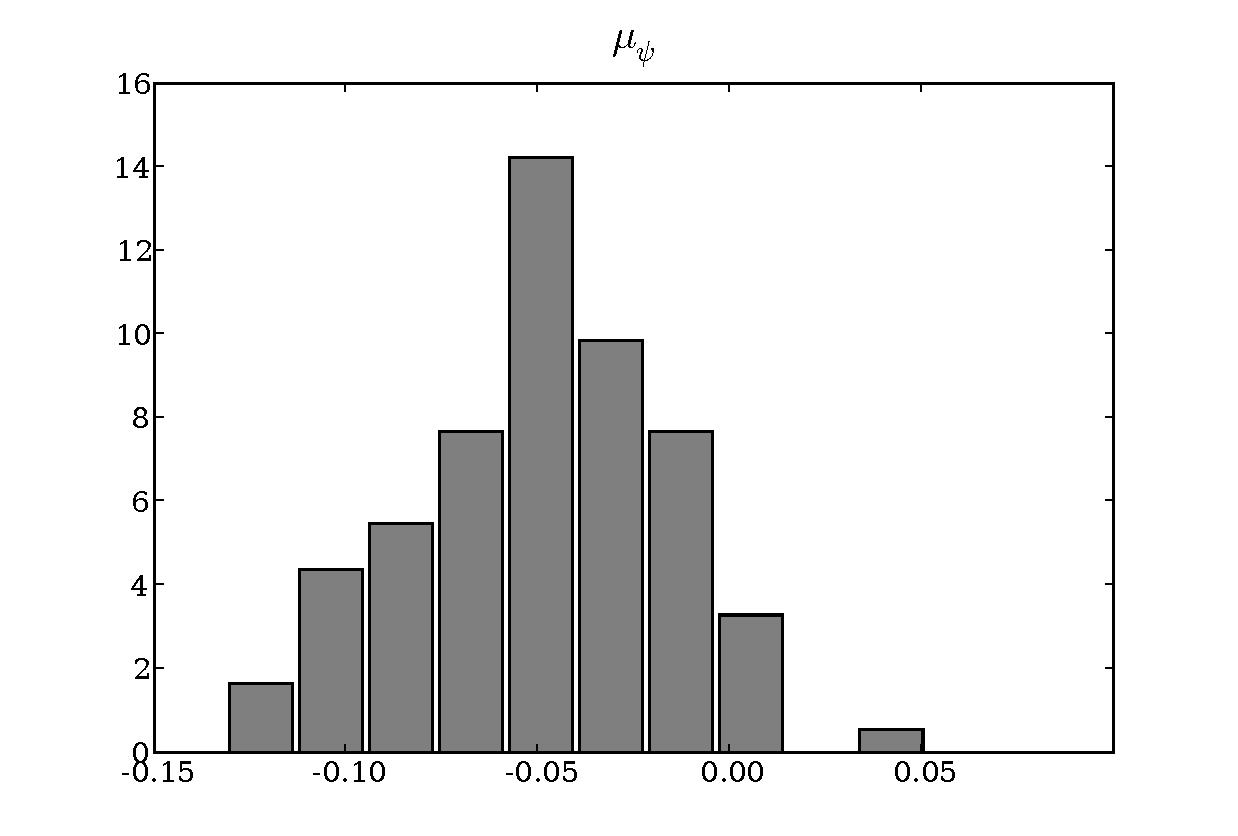
\epsfig{file=figs/ESSmupsiPosterior.pdf,width=7cm}
% % %         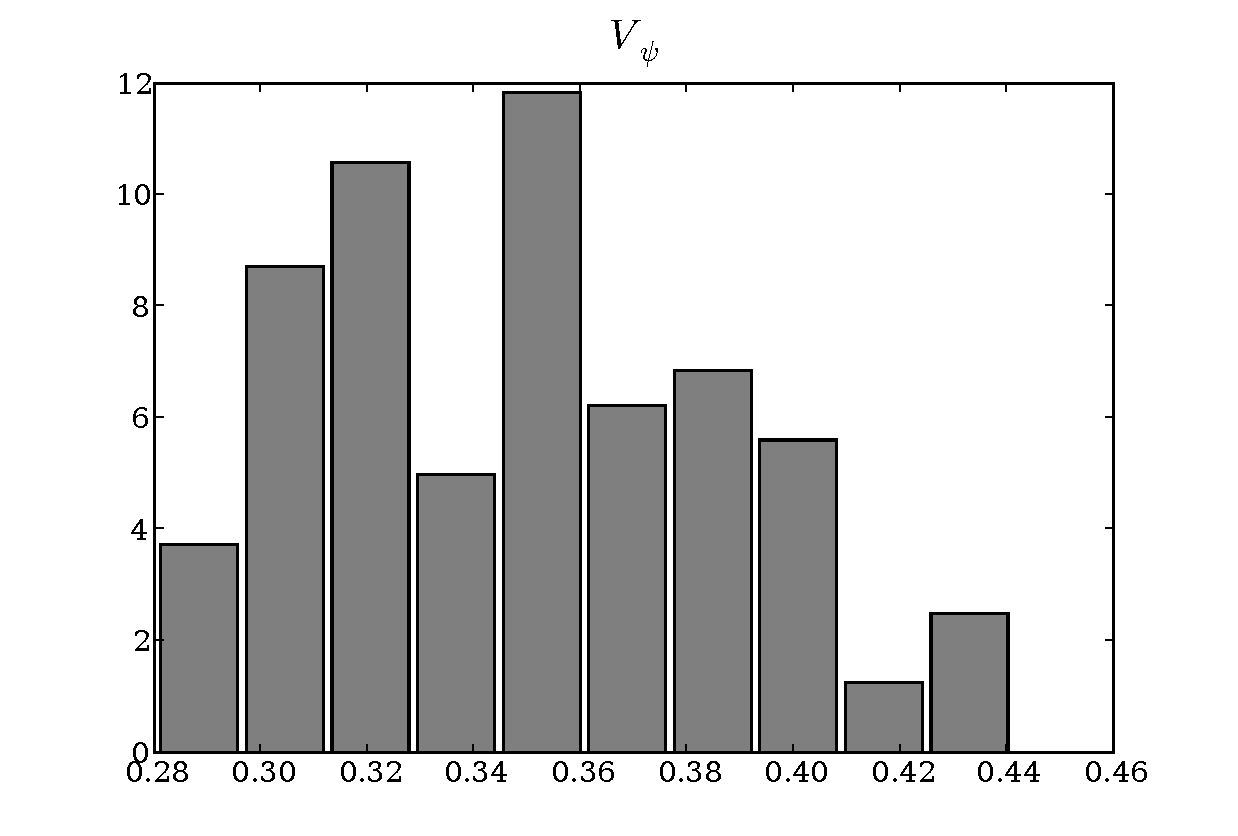
\epsfig{file=figs/ESSVpsiPosterior.pdf,width=7cm}
% % %     \caption{caption}
% % %     \label{fig:ESSphipsi}
% % % \end{figure}
% % %
% % % \begin{figure}
% % %     \centering
% % %         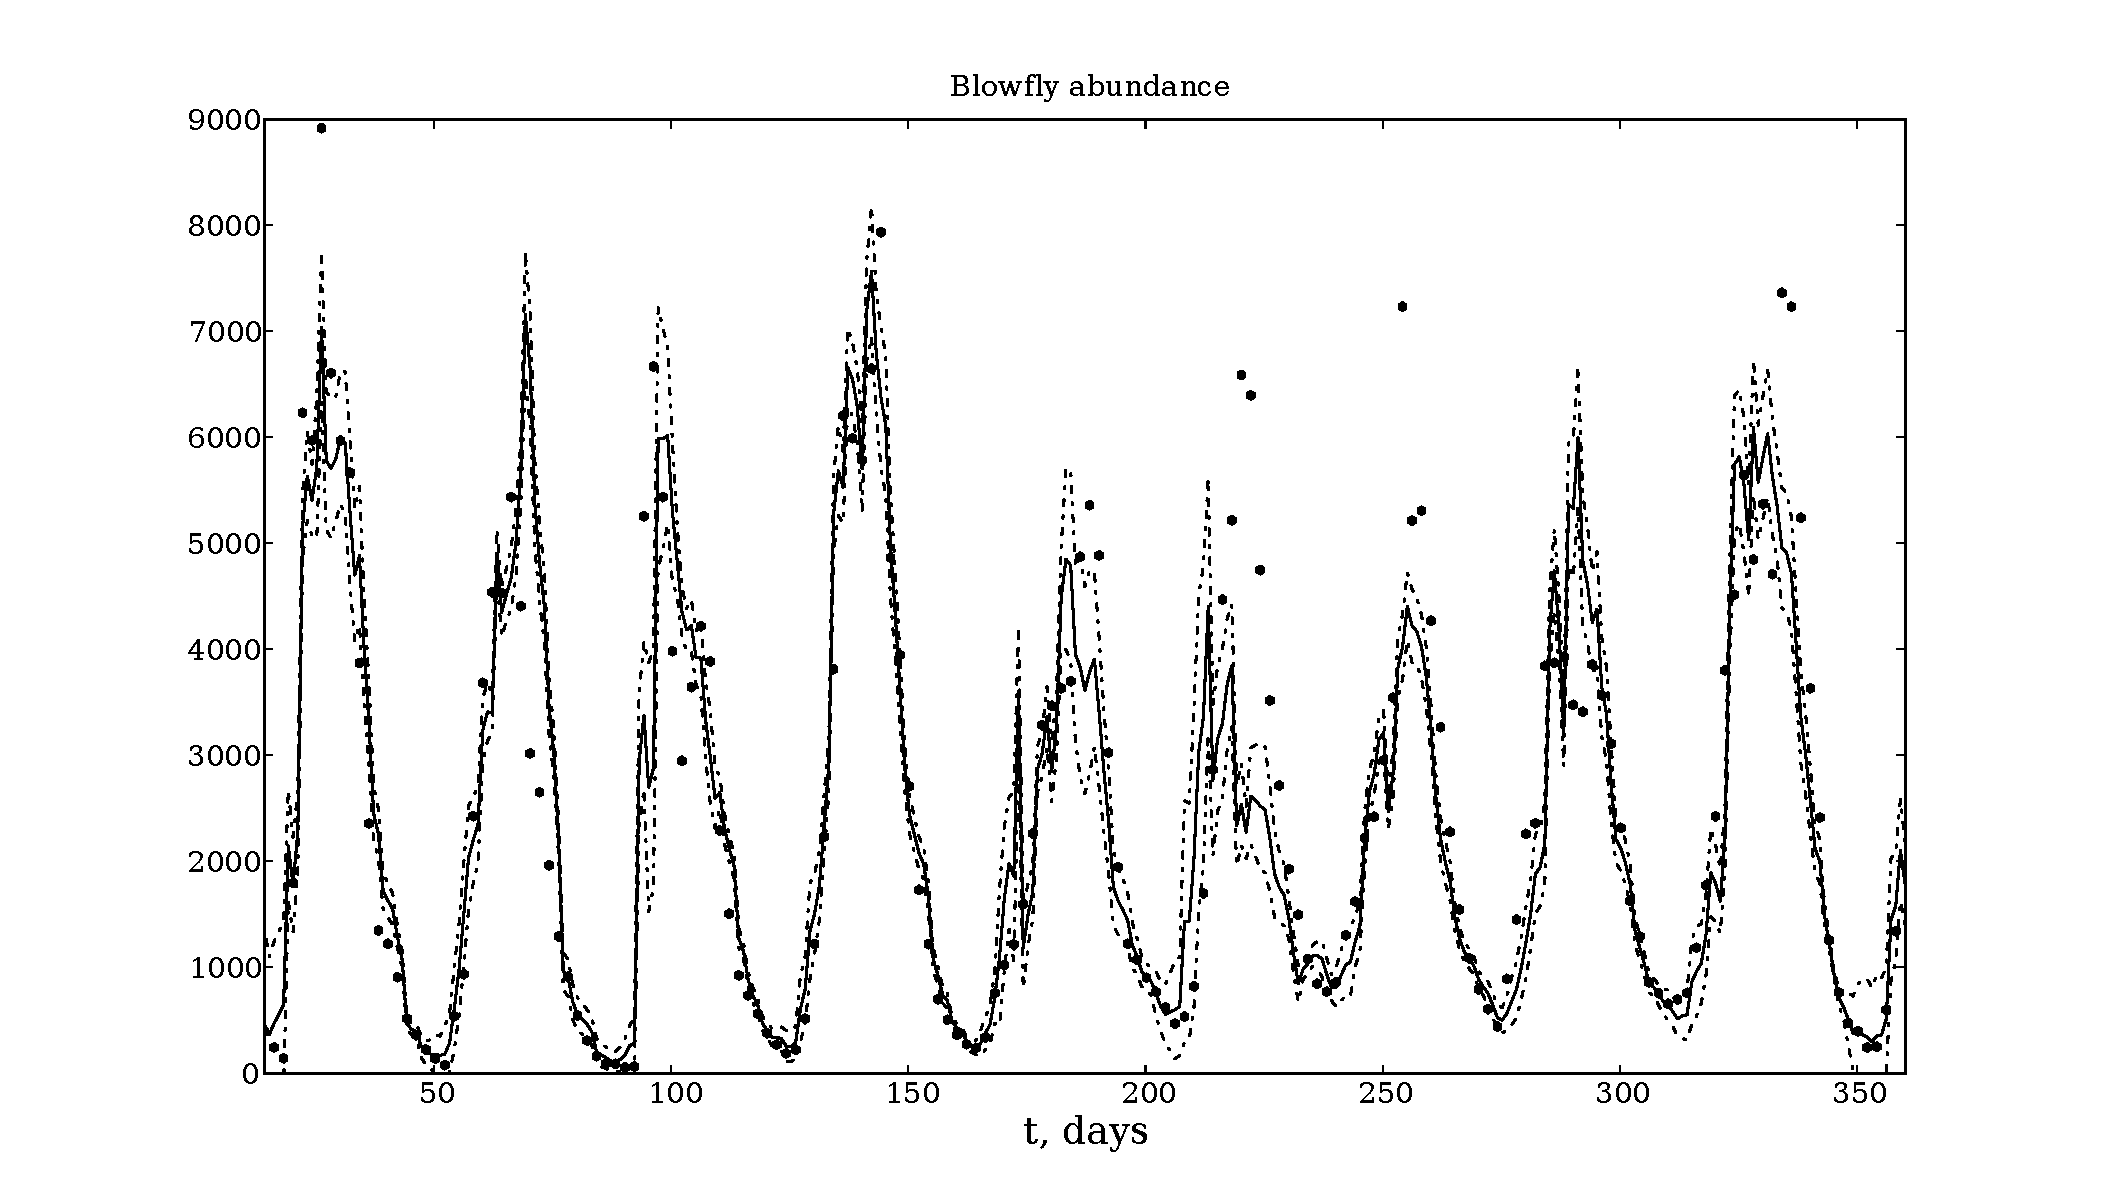
\epsfig{file=figs/ESSblowflyfit.pdf,width=15cm}
% % %     \caption{caption}
% % %     \label{fig:ESSfit}
% % % \end{figure}
% %
